\documentclass{article}
\usepackage{graphicx}
 
\usepackage{graphicx}
\usepackage{ifpdf}

\ifpdf
  \DeclareGraphicsRule{*}{mps}{*}{}
\fi

\usepackage{subfigure}

\begin{document}


\begin{figure}%[htp]
     \centering
     \subfigure[f]{
          \label{fig:ellipse_a}
          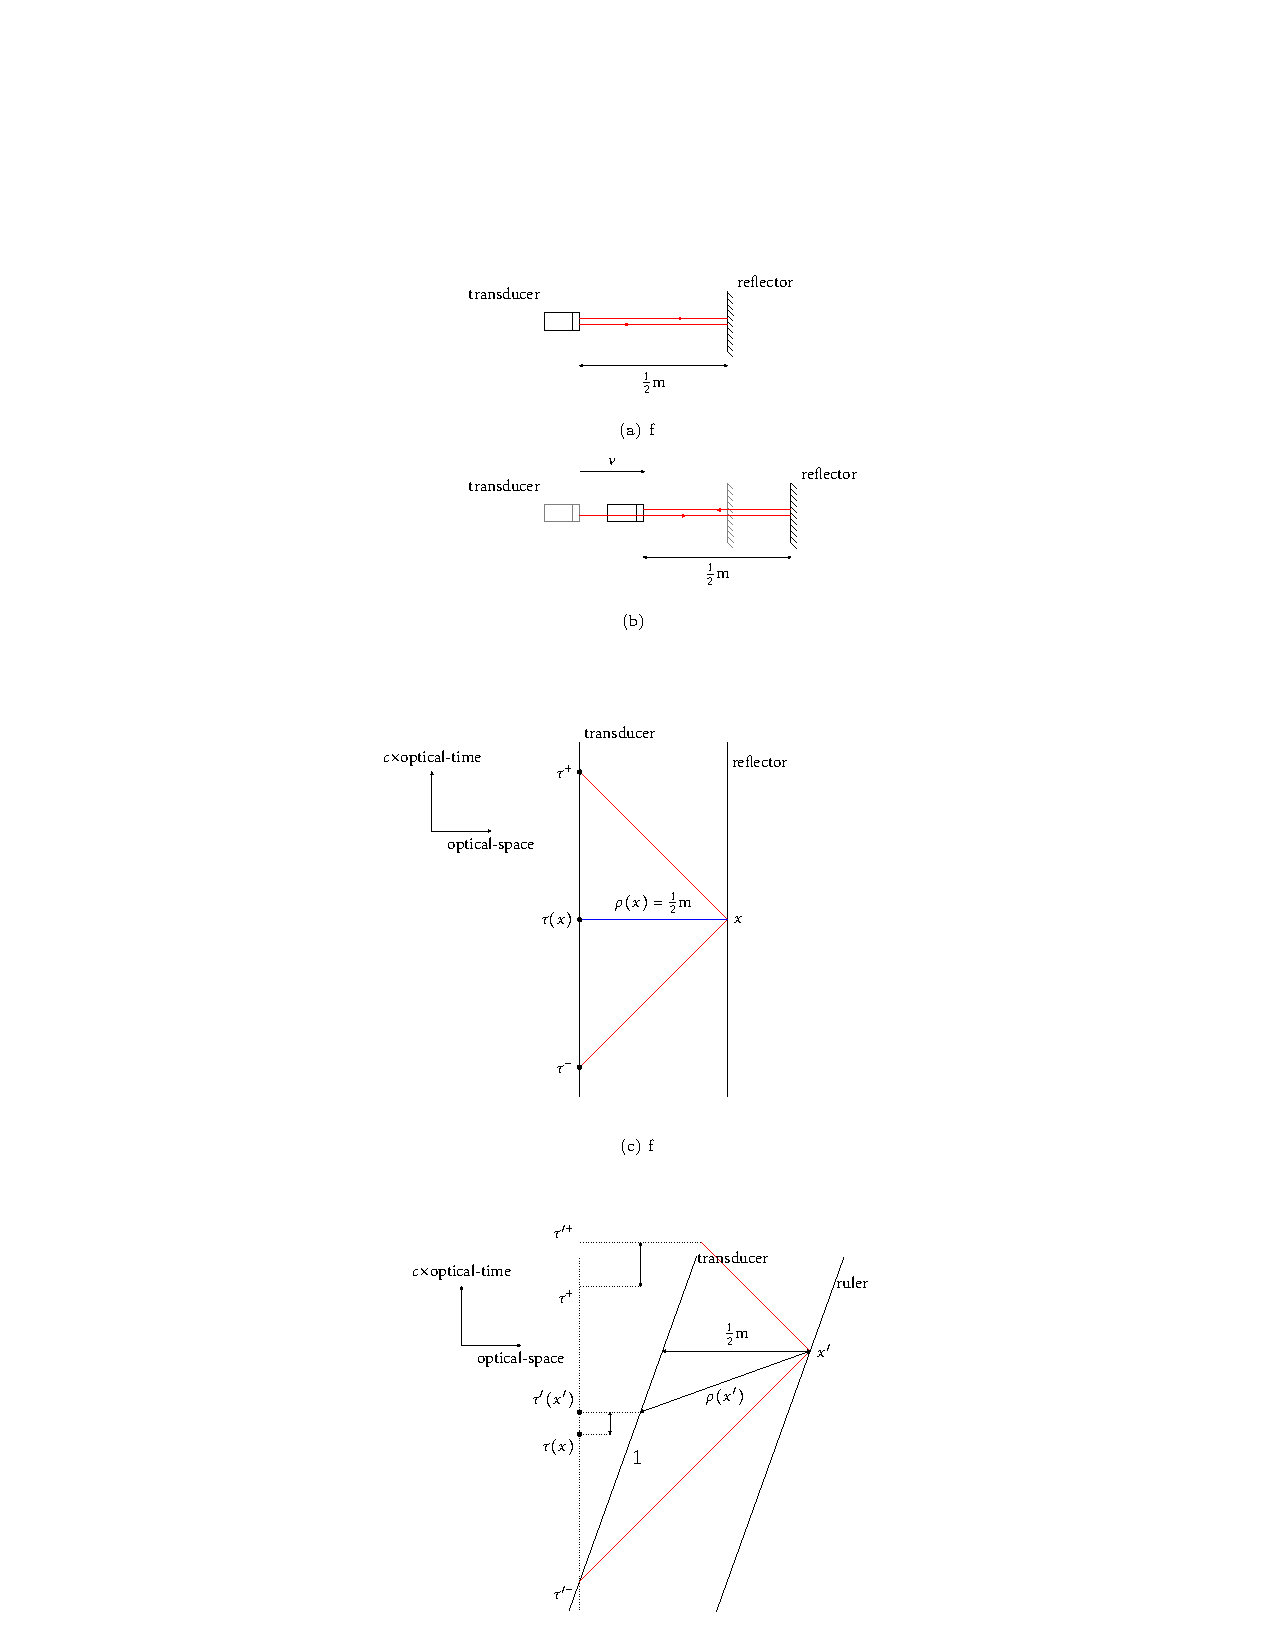
\includegraphics{measurement_figs.0}}
     \hspace{1cm}
     \subfigure[]{
          \label{fig:ellipse_b}
          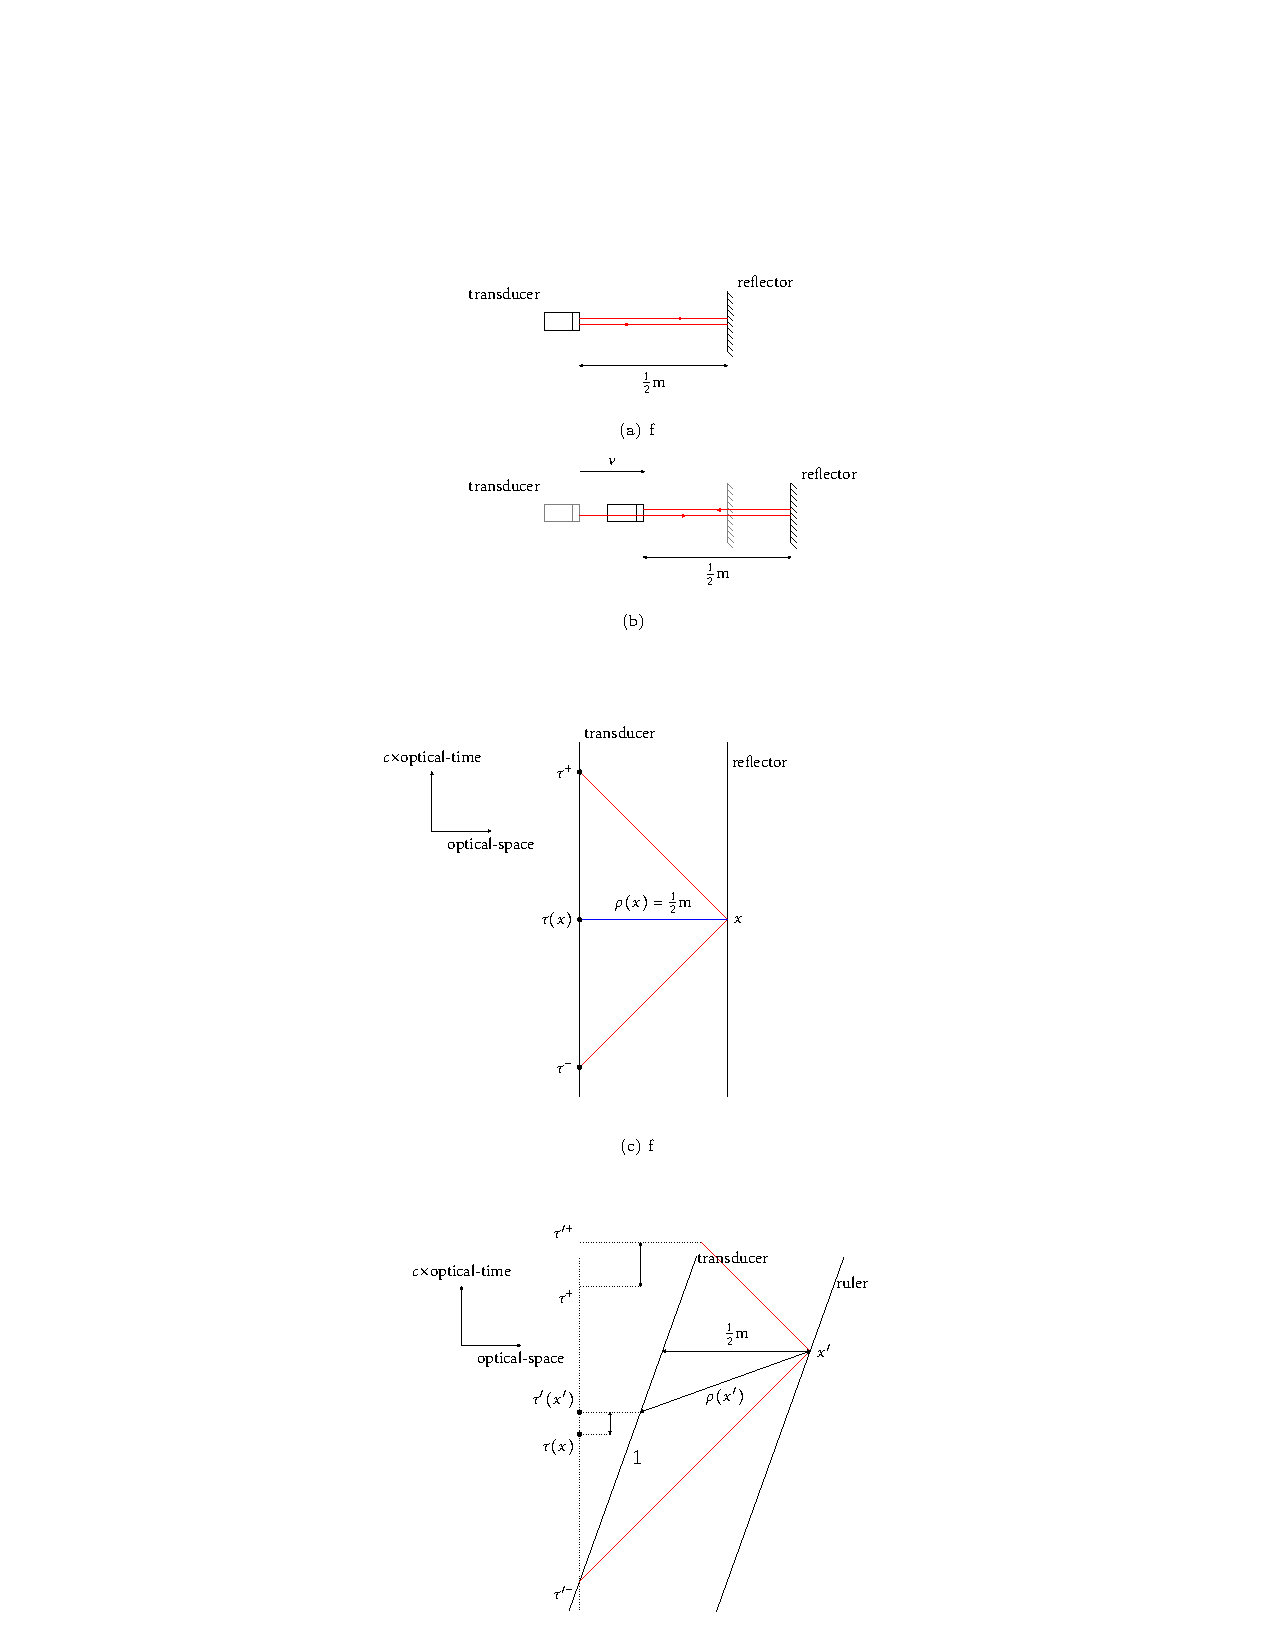
\includegraphics{measurement_figs.1}}
\\
    \subfigure[f]{
          \label{fig:ellipse_a}
          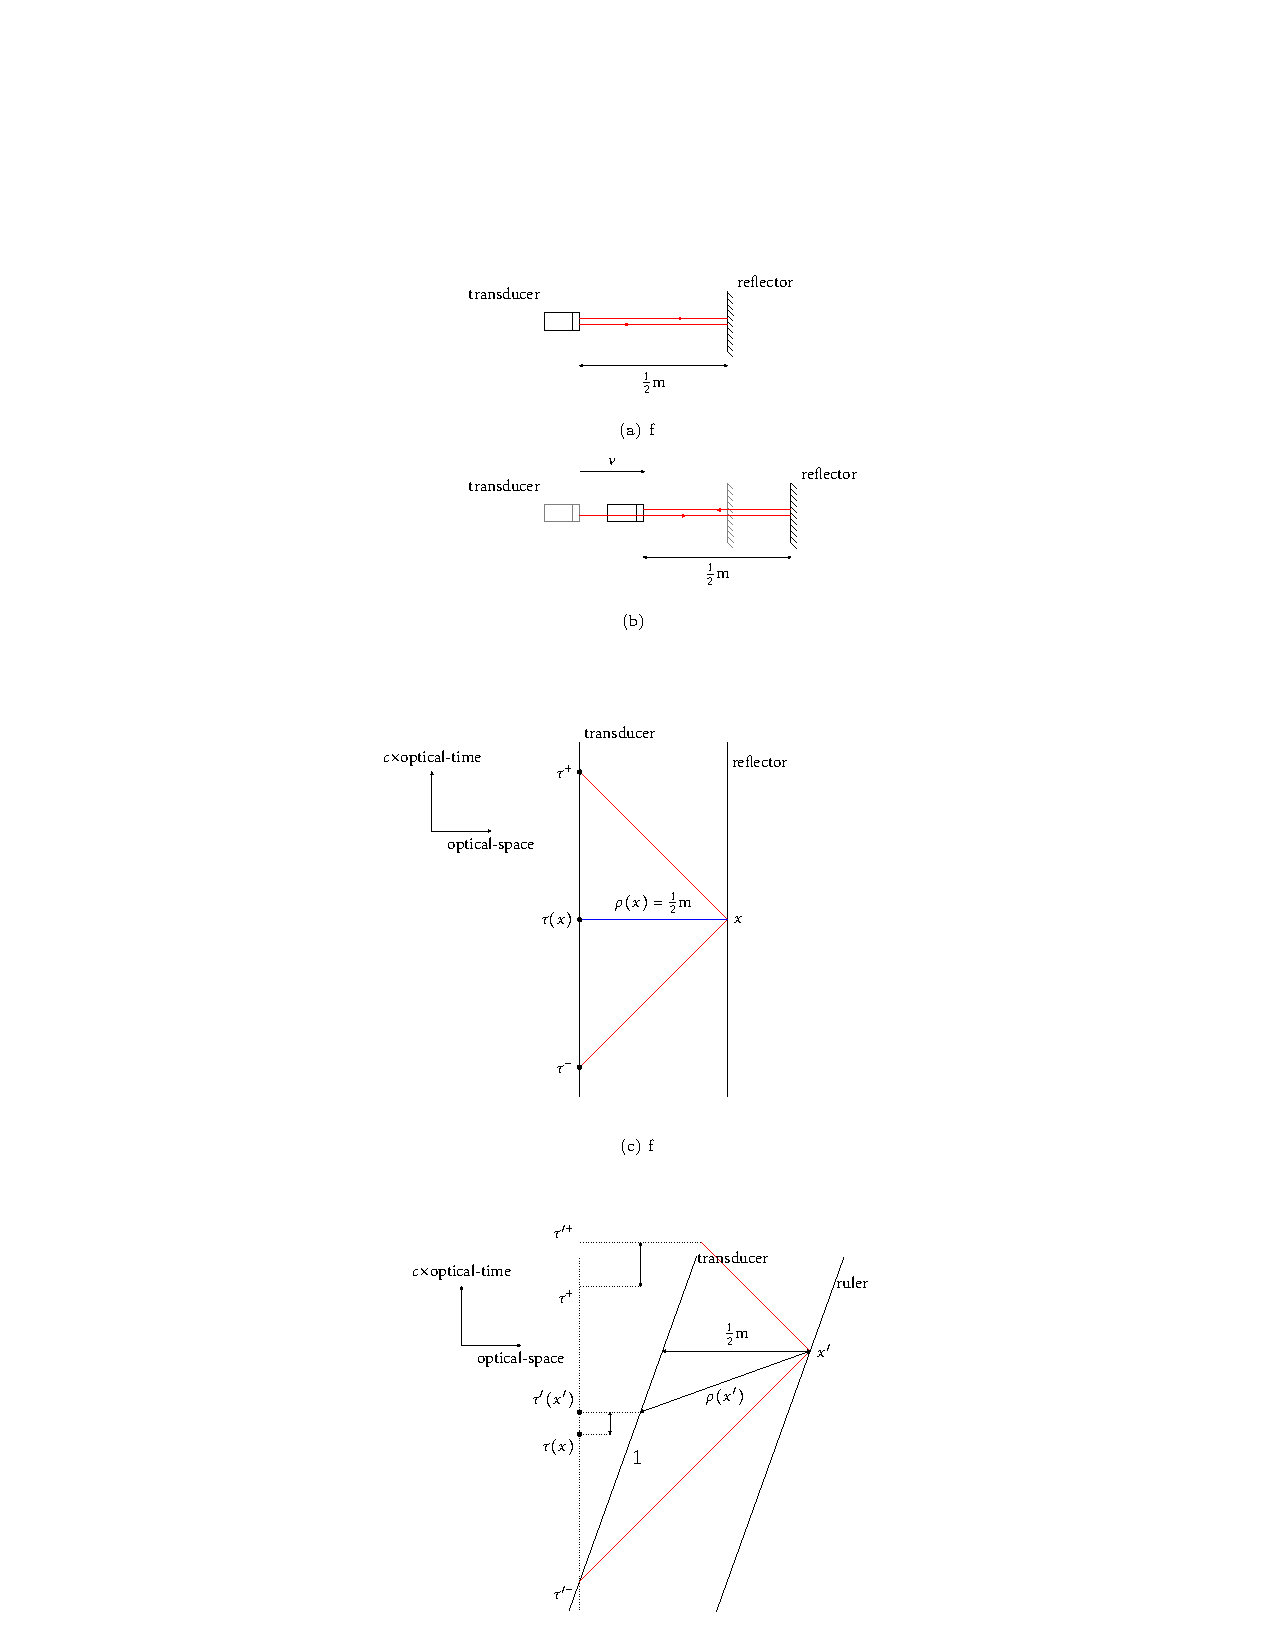
\includegraphics{measurement_figs.2}}
     \hspace{1cm}
     \subfigure[]{
          \label{fig:ellipse_b}
          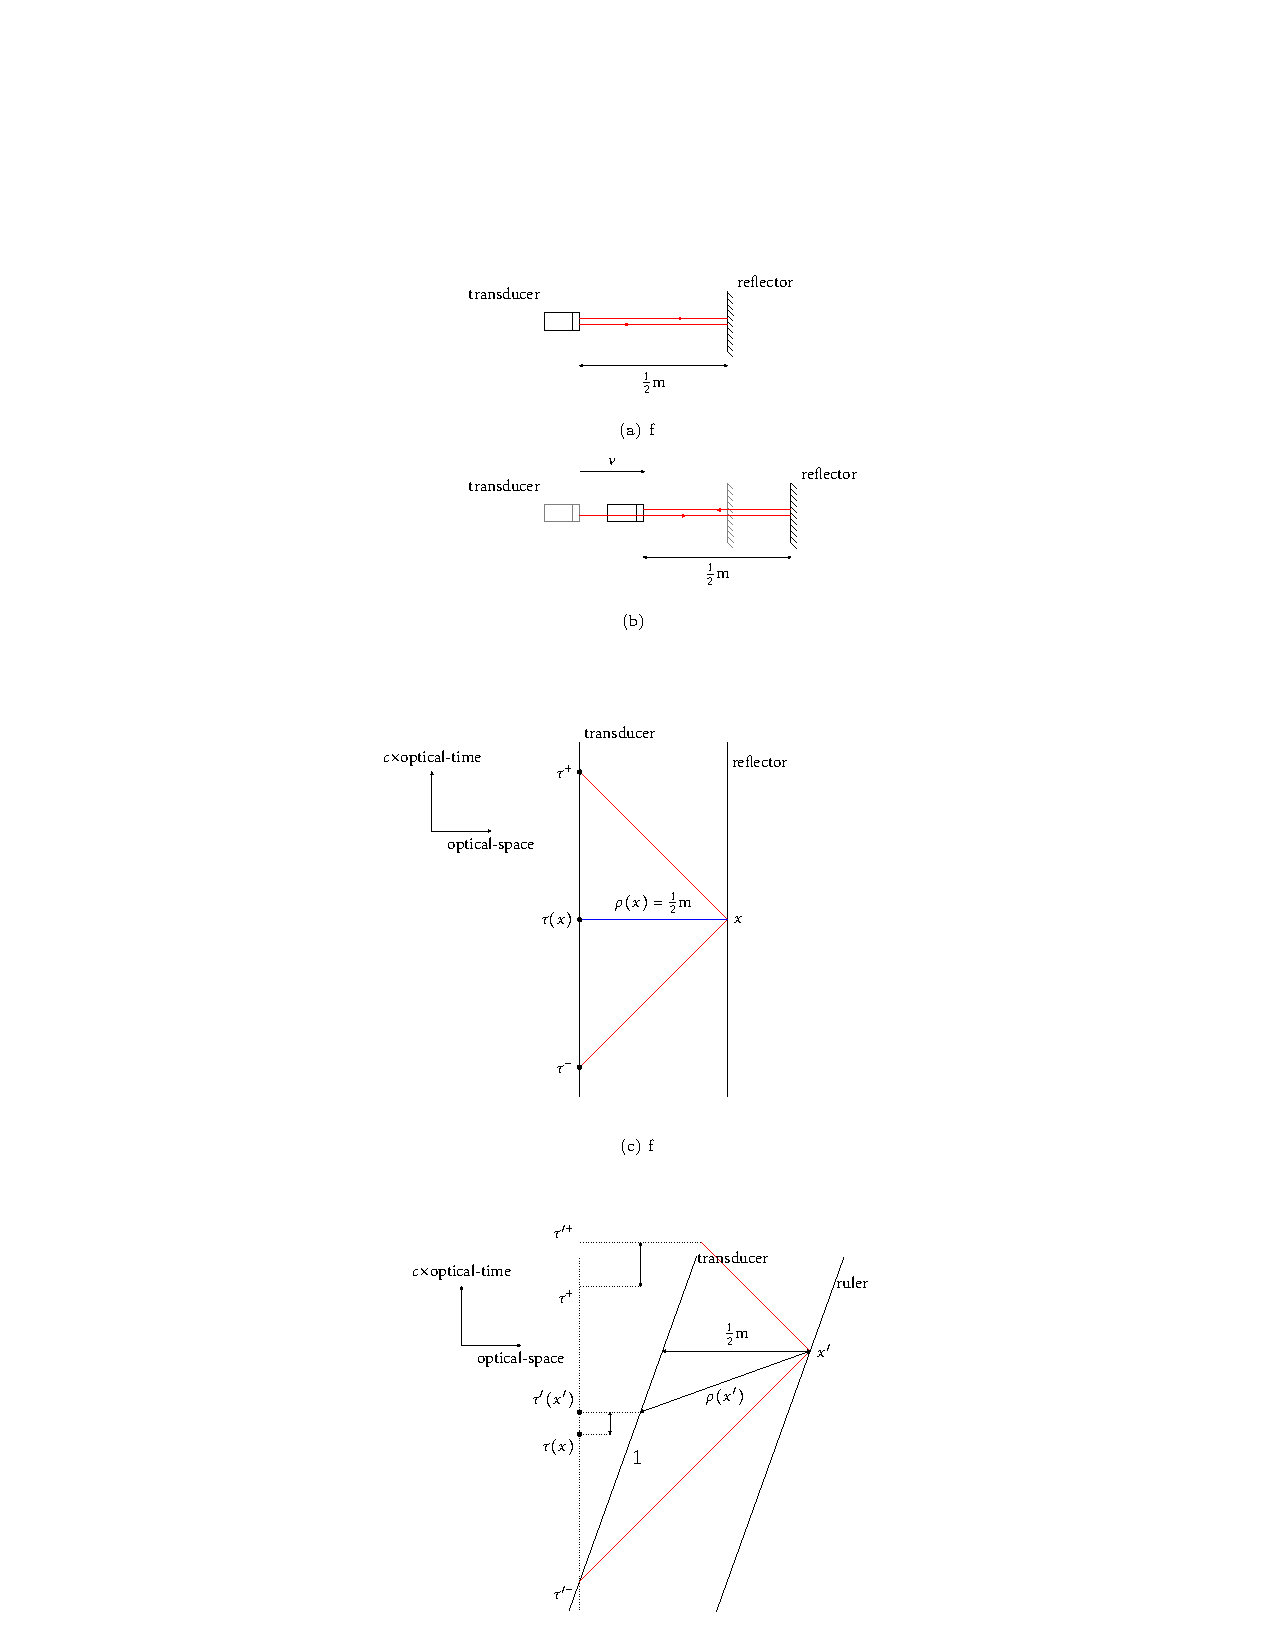
\includegraphics{measurement_figs.3}}
     \caption{caption}
     \label{fig:ellipse}
\end{figure}



\begin{figure}%[htp]
     \centering
    \subfigure[f]{
          \label{fig:ellipse_a}
          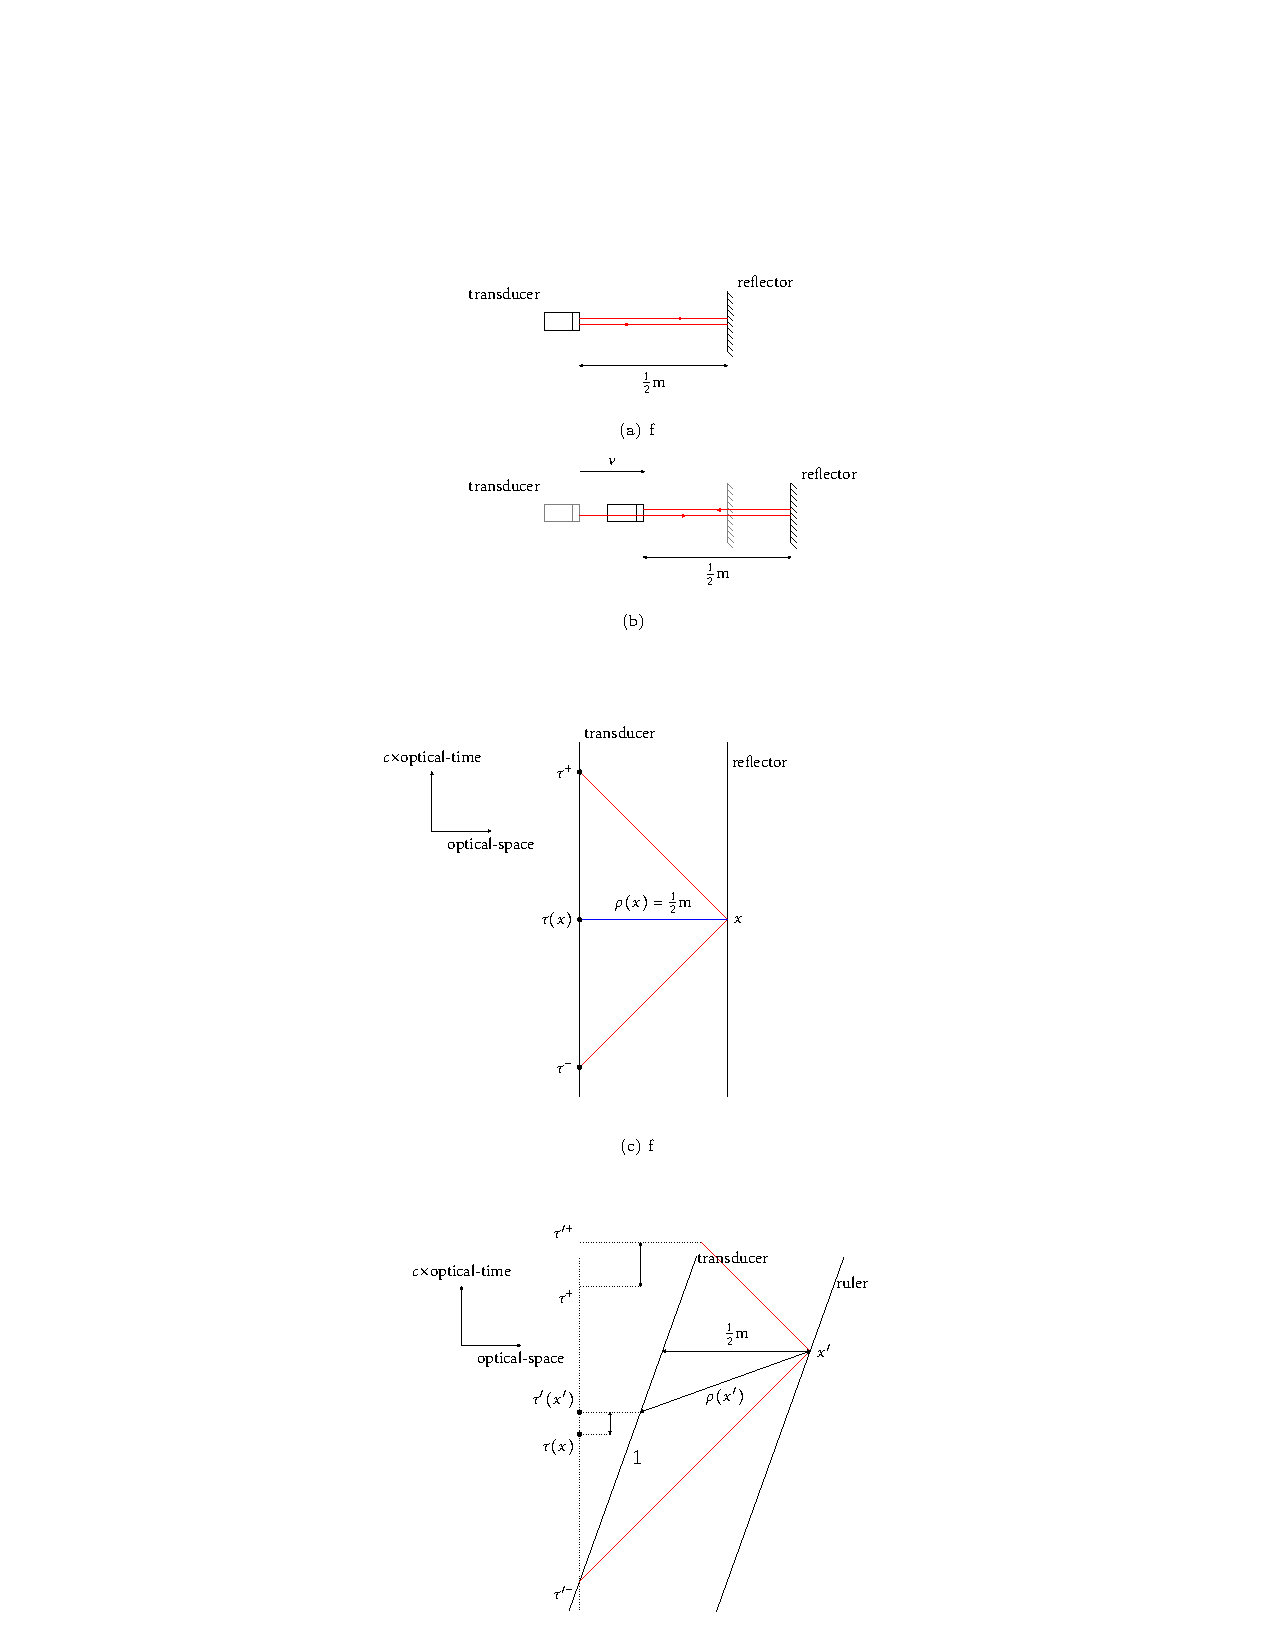
\includegraphics{measurement_figs.4}}
     \caption{caption}
     \label{fig:ellipse}
\end{figure}



\begin{figure}%[htp]
     \centering
    \subfigure[f]{
          \label{fig:ellipse_a}
          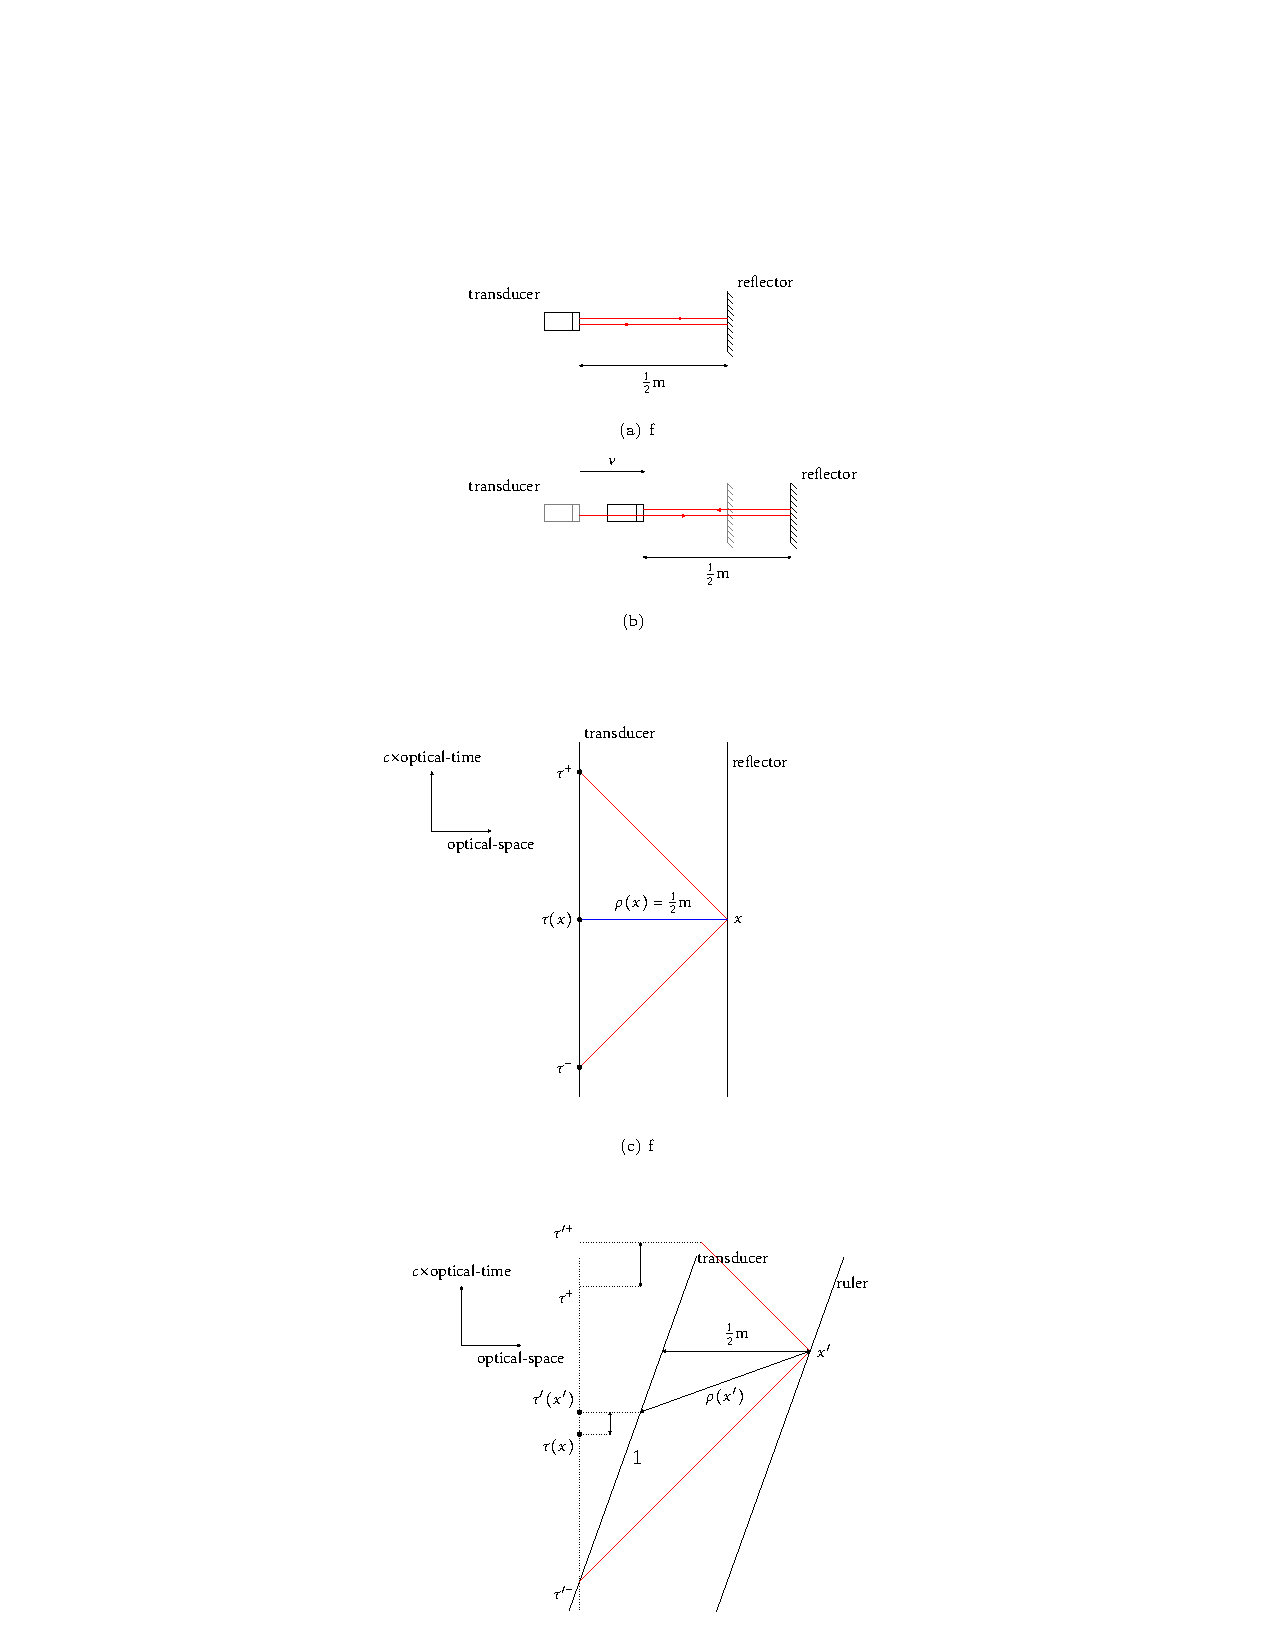
\includegraphics{measurement_figs.5}}
     \hspace{3cm}
     \label{fig:ellipse}
\end{figure}


\begin{figure}%[htp]
     \centering
     \subfigure[f]{
          \label{fig:ellipse_a}
          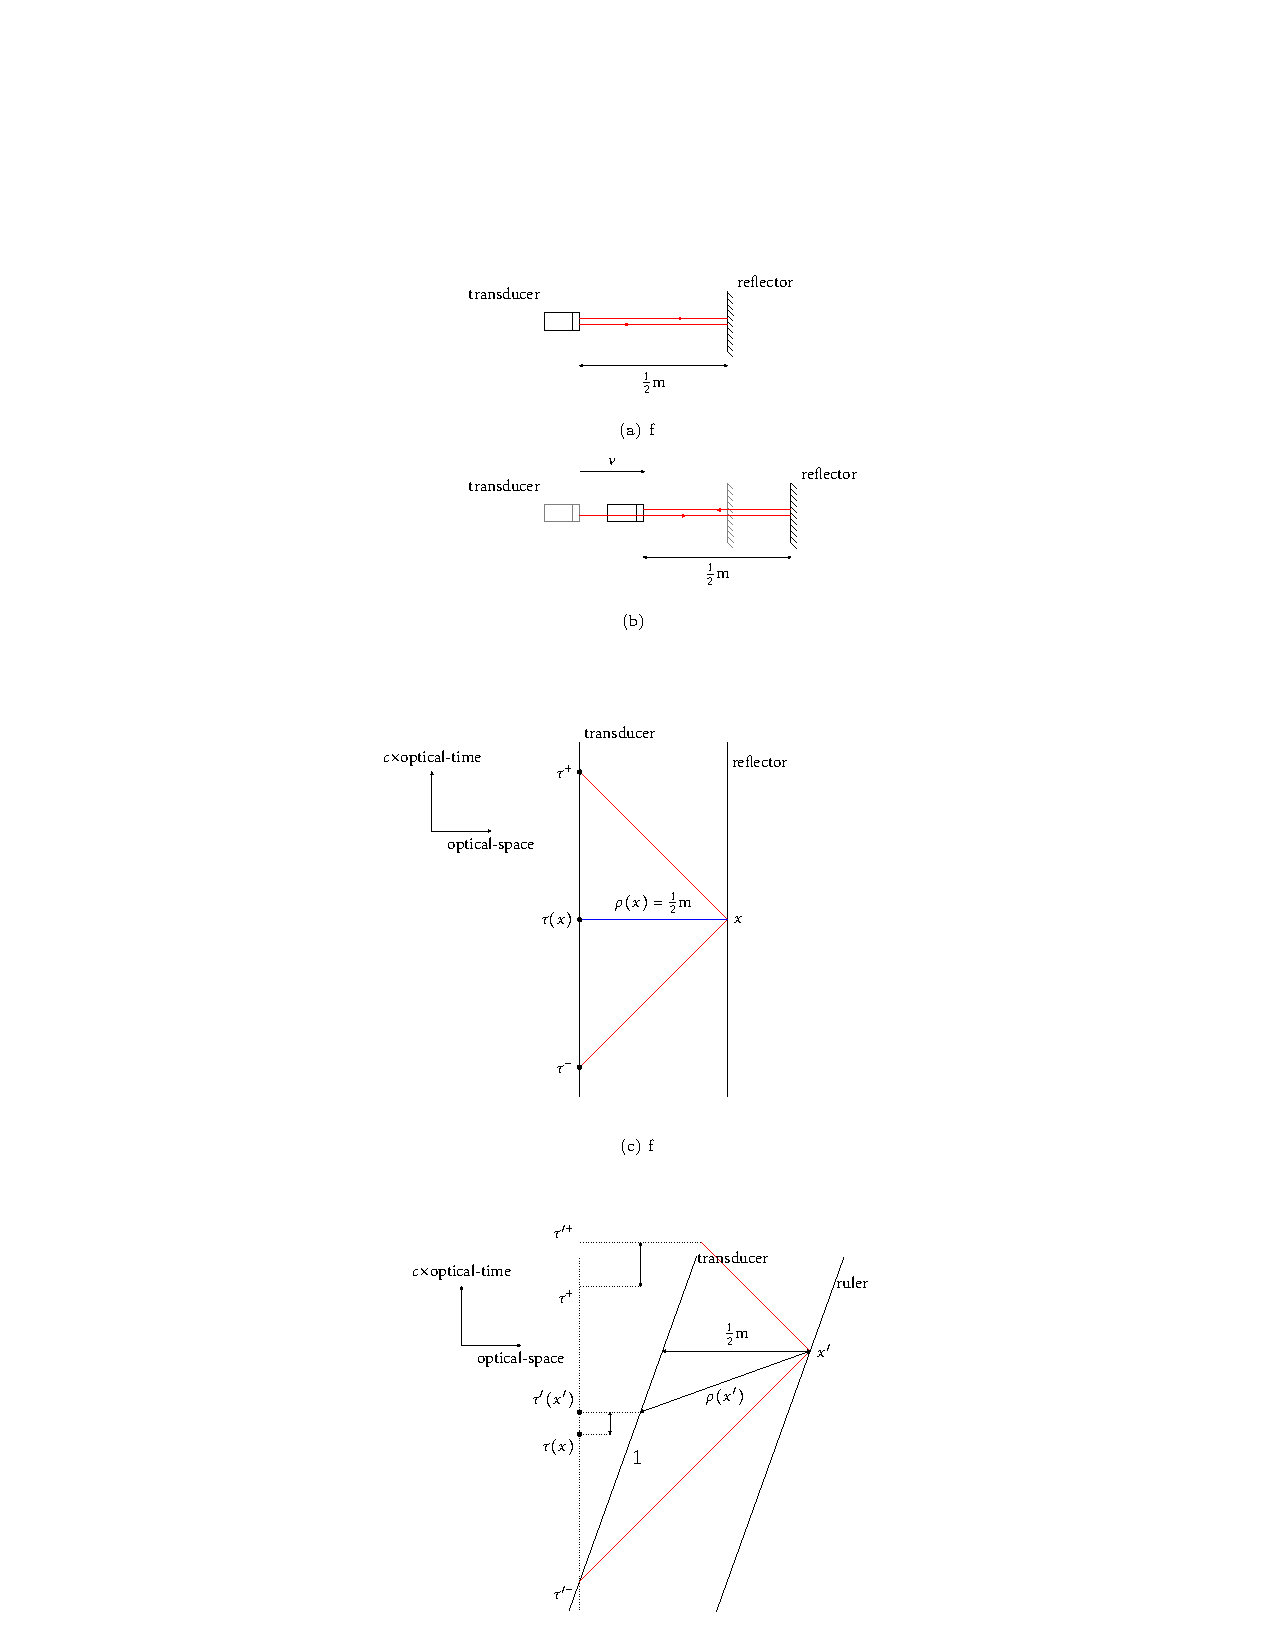
\includegraphics{measurement_figs.6}}
        \\
    \subfigure[f]{
          \label{fig:ellipse_a}
          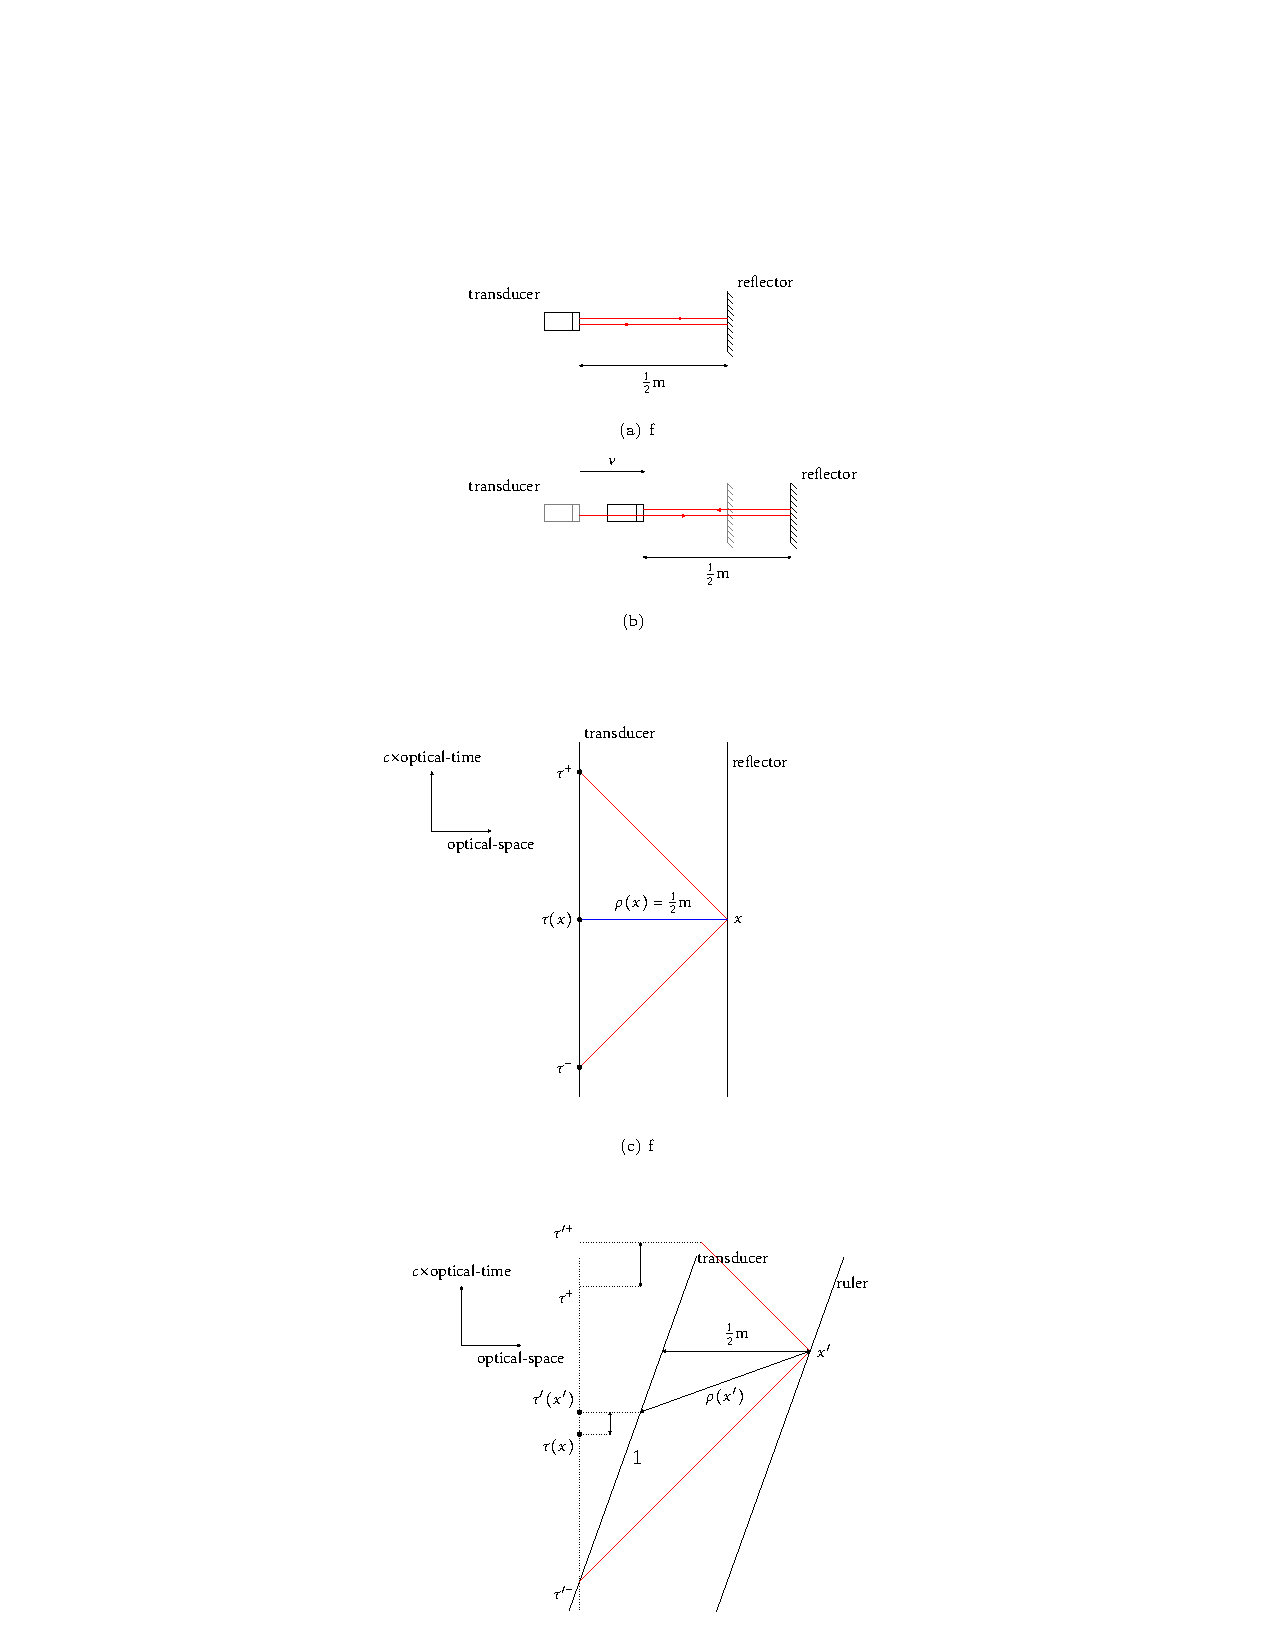
\includegraphics{measurement_figs.7}}
         \caption{caption}
     \label{fig:ellipse}
\end{figure}



% \begin{figure}%[htp]
%      \centering
%      \subfigure[f]{
%           \label{fig:ellipse_a}
%           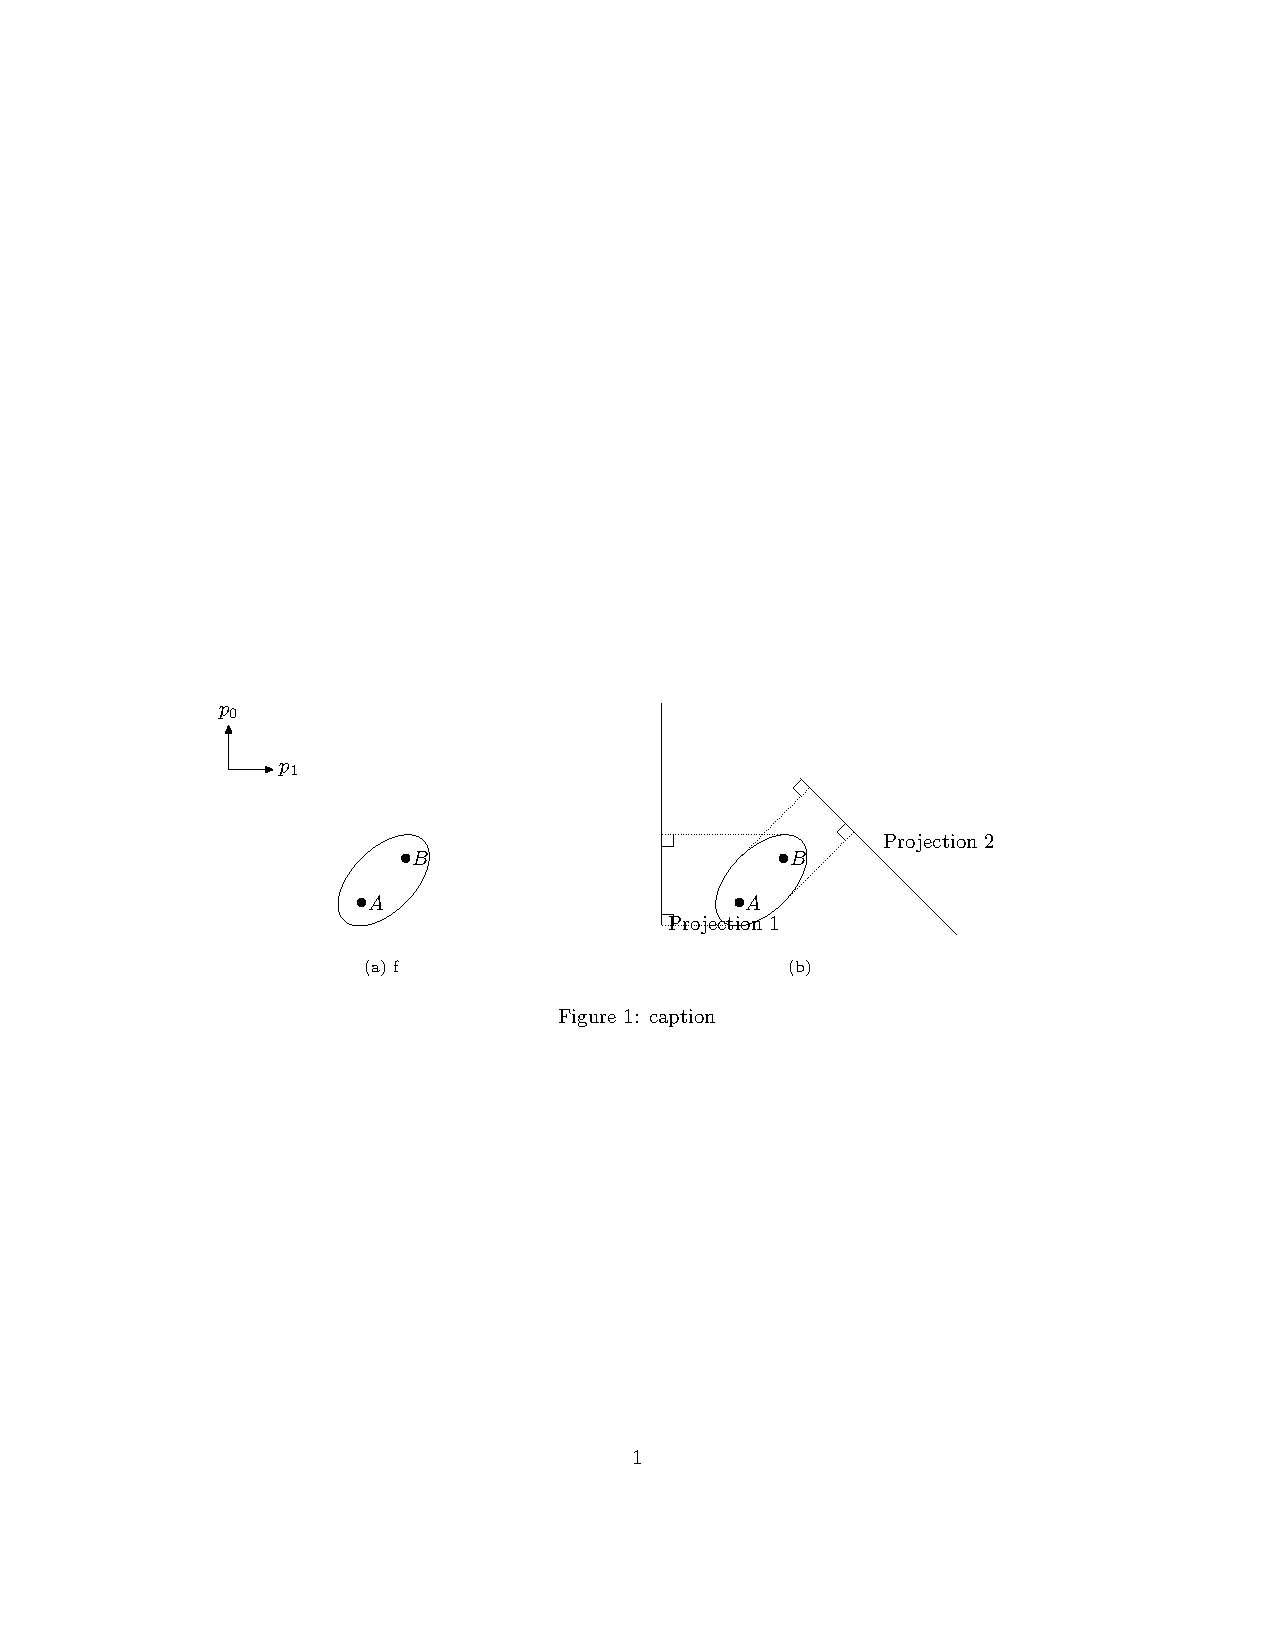
\includegraphics{measurement.2}}
%      \hspace{3cm}
%      \subfigure[]{
%           \label{fig:ellipse_b}
%           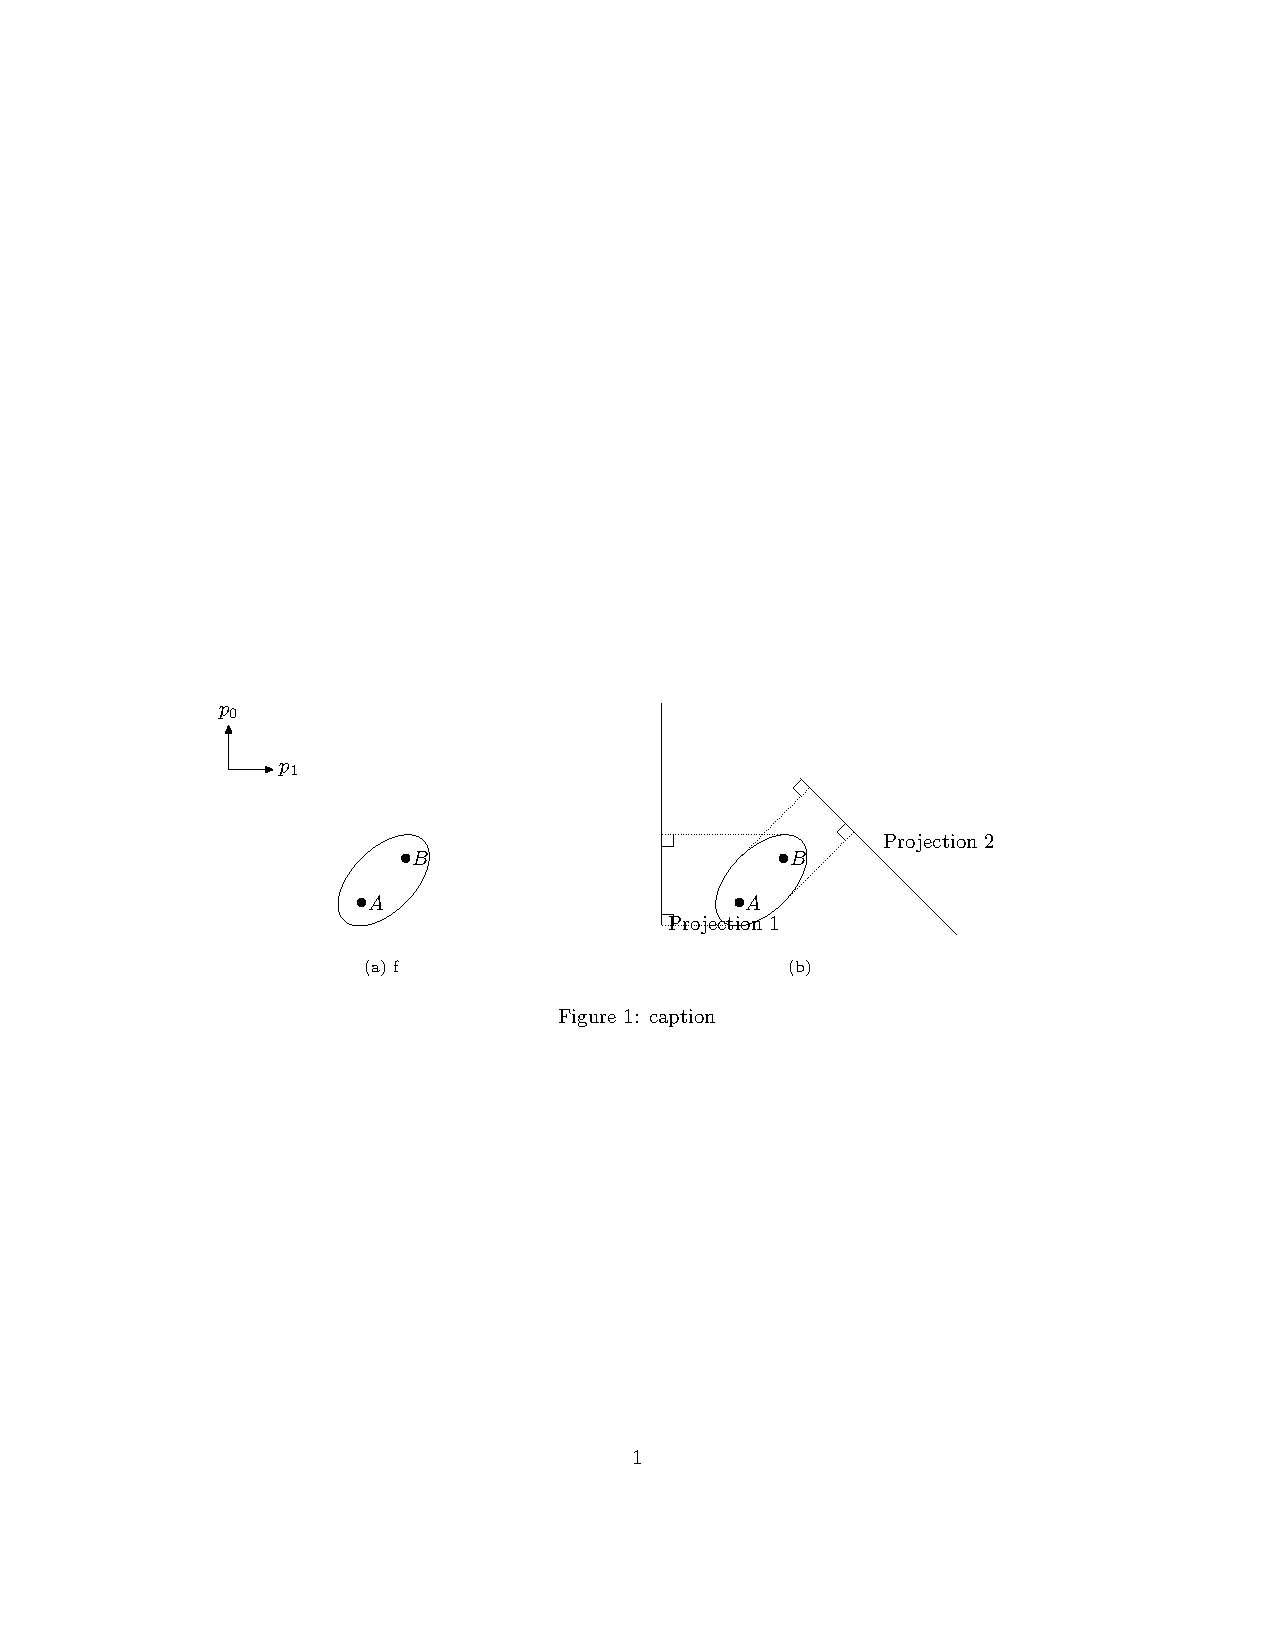
\includegraphics{measurement.11}}
    
%      \caption{caption}
%      \label{fig:ellipse}
% \end{figure}

% \begin{figure}%[htp]
%  \centering
%  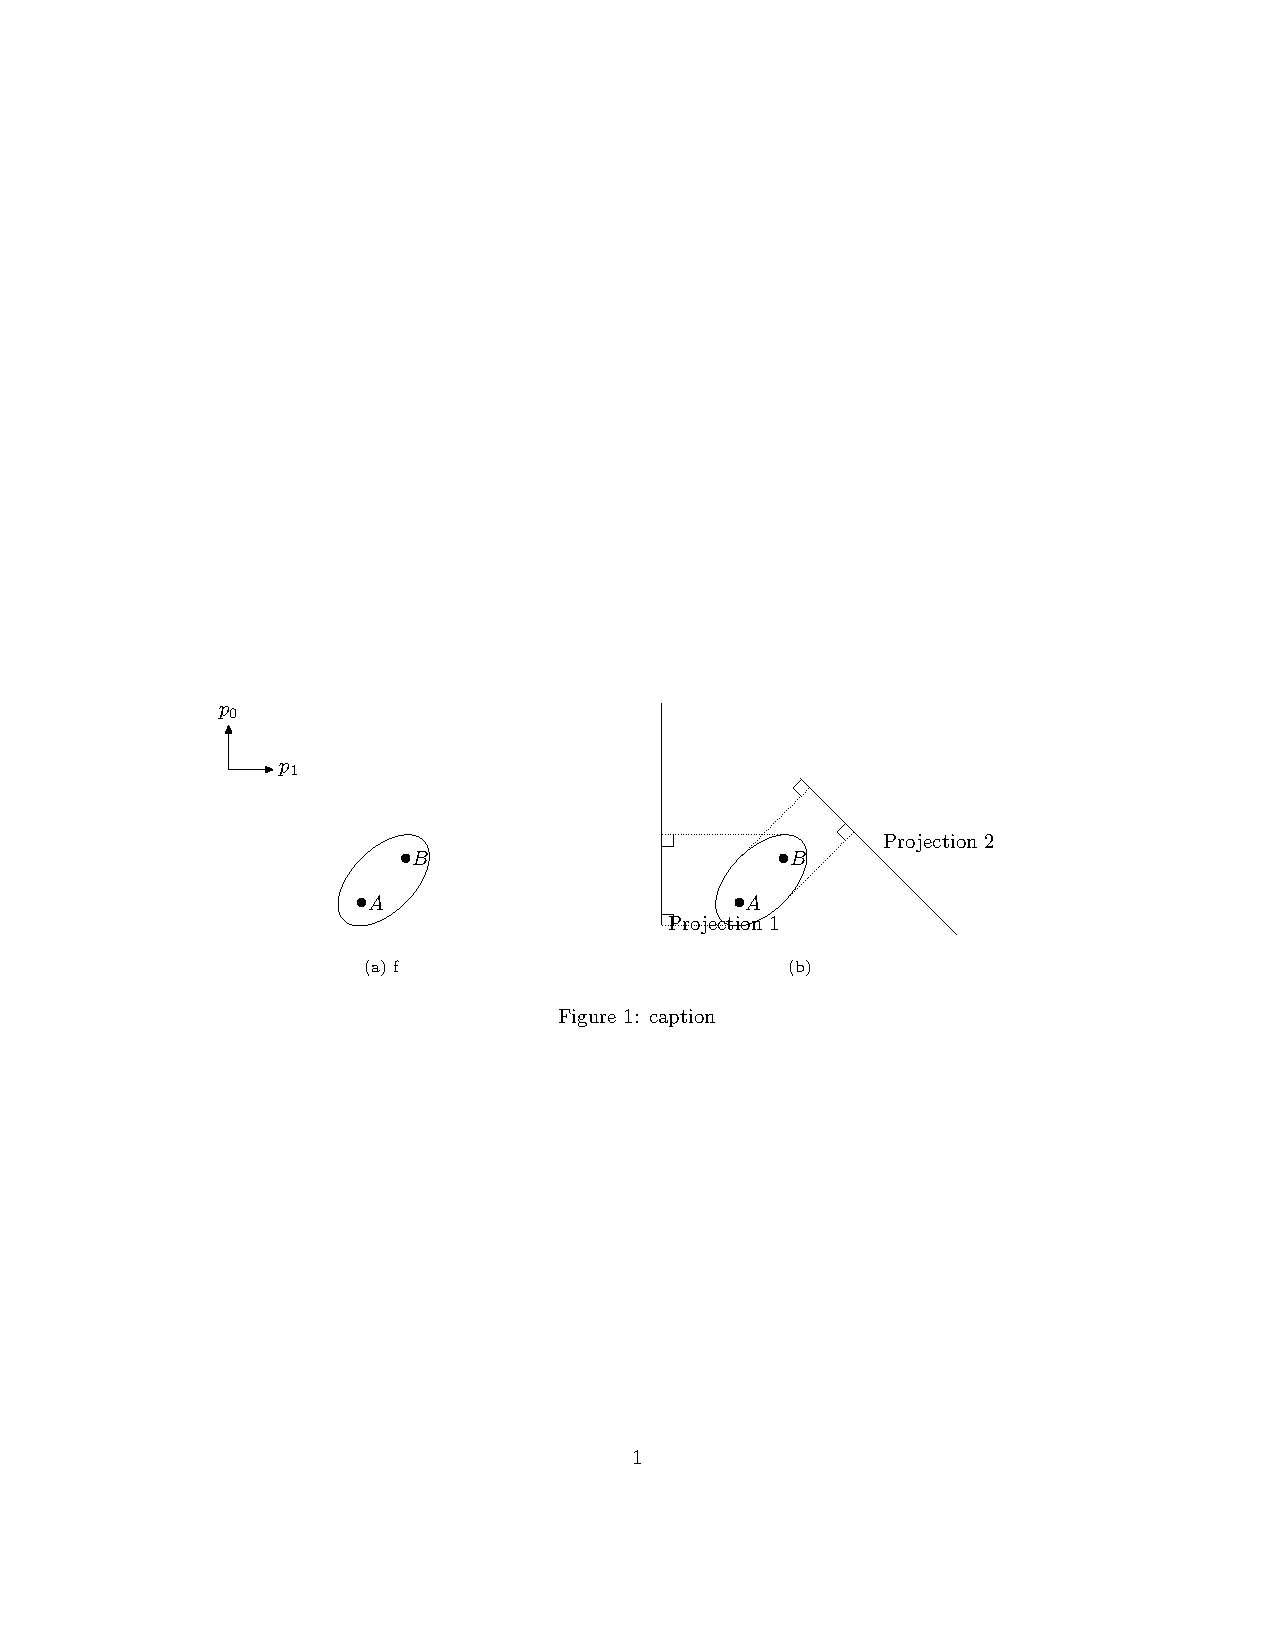
\includegraphics{measurement.2}
%  \caption{caption}
%  \label{fig:ObsEuclid}
% \end{figure}

% \begin{figure}%[htp]
%      \centering
%      \subfigure[]{
%           \label{fig:ObsA}
%           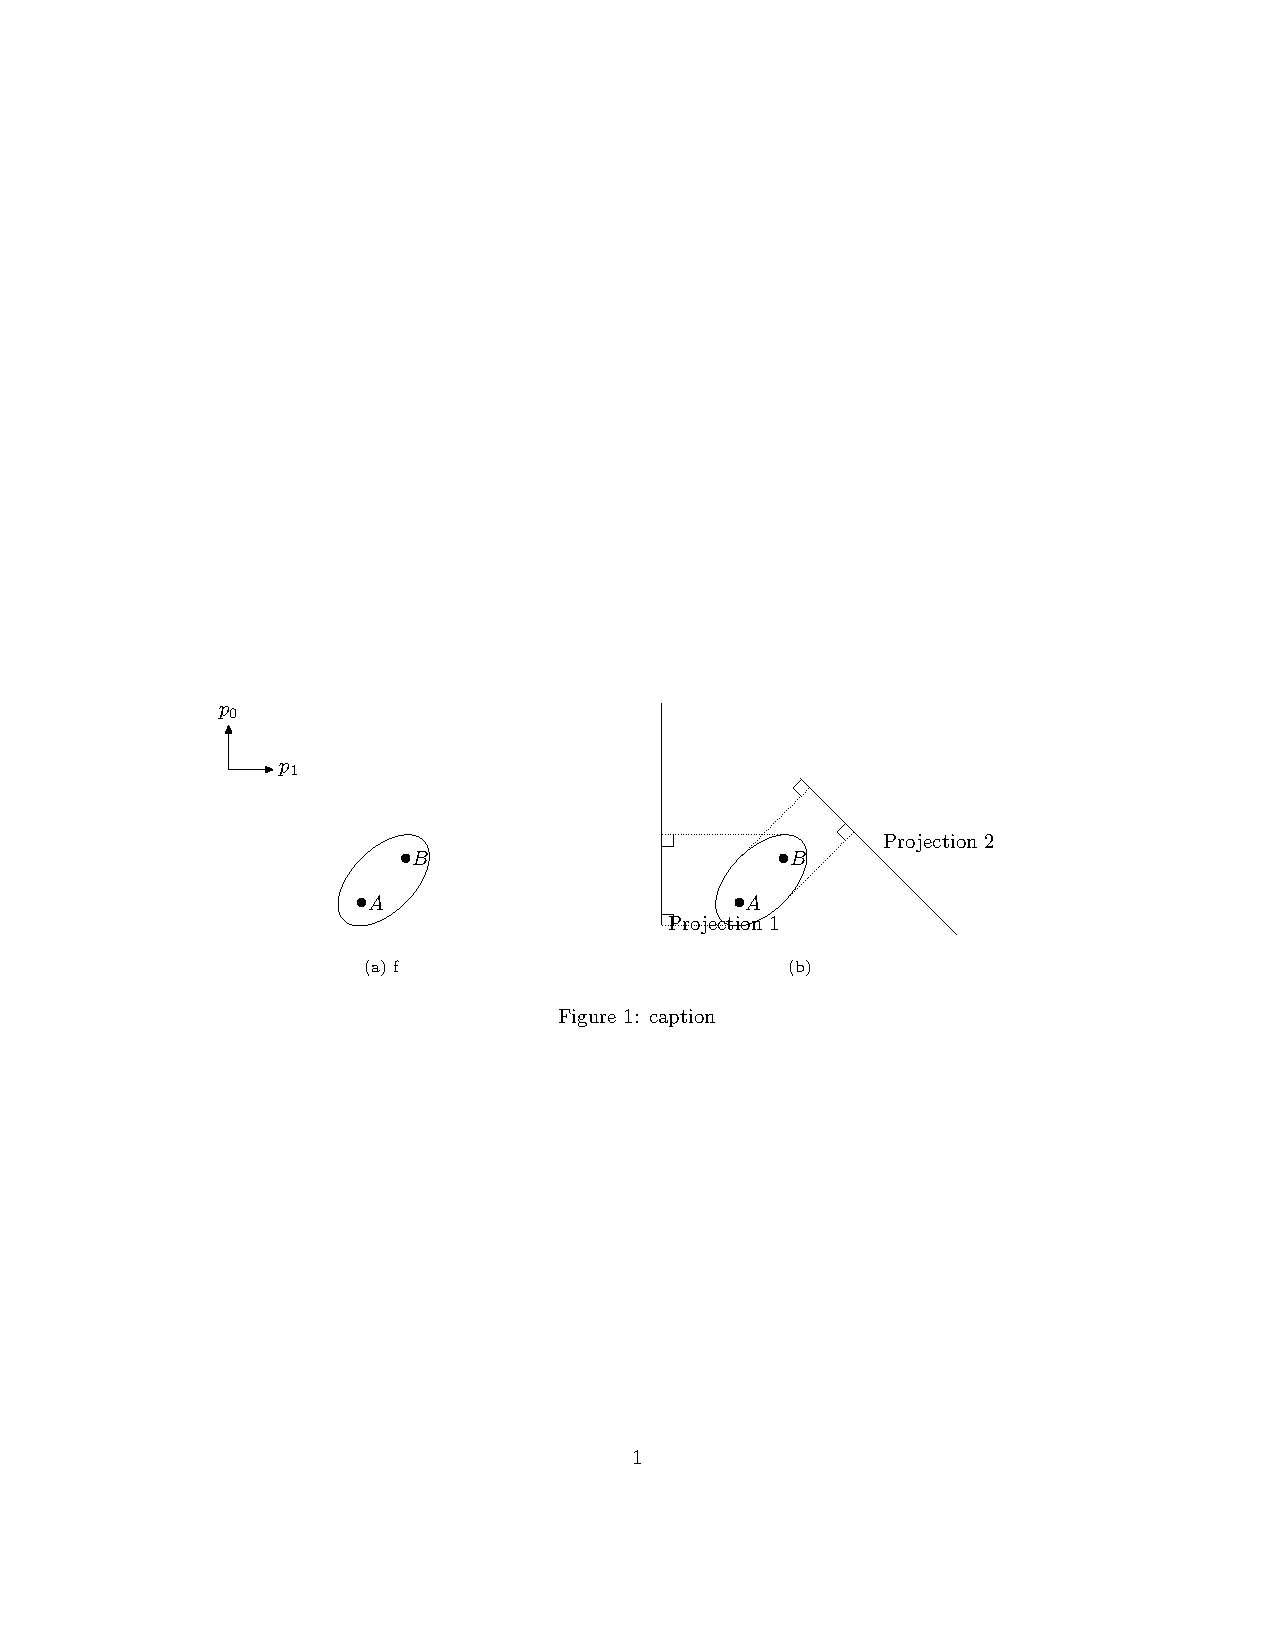
\includegraphics{measurement.3}}
%      \hspace{1cm}
%      \subfigure[]{
%           \label{fig:ObsB}
%           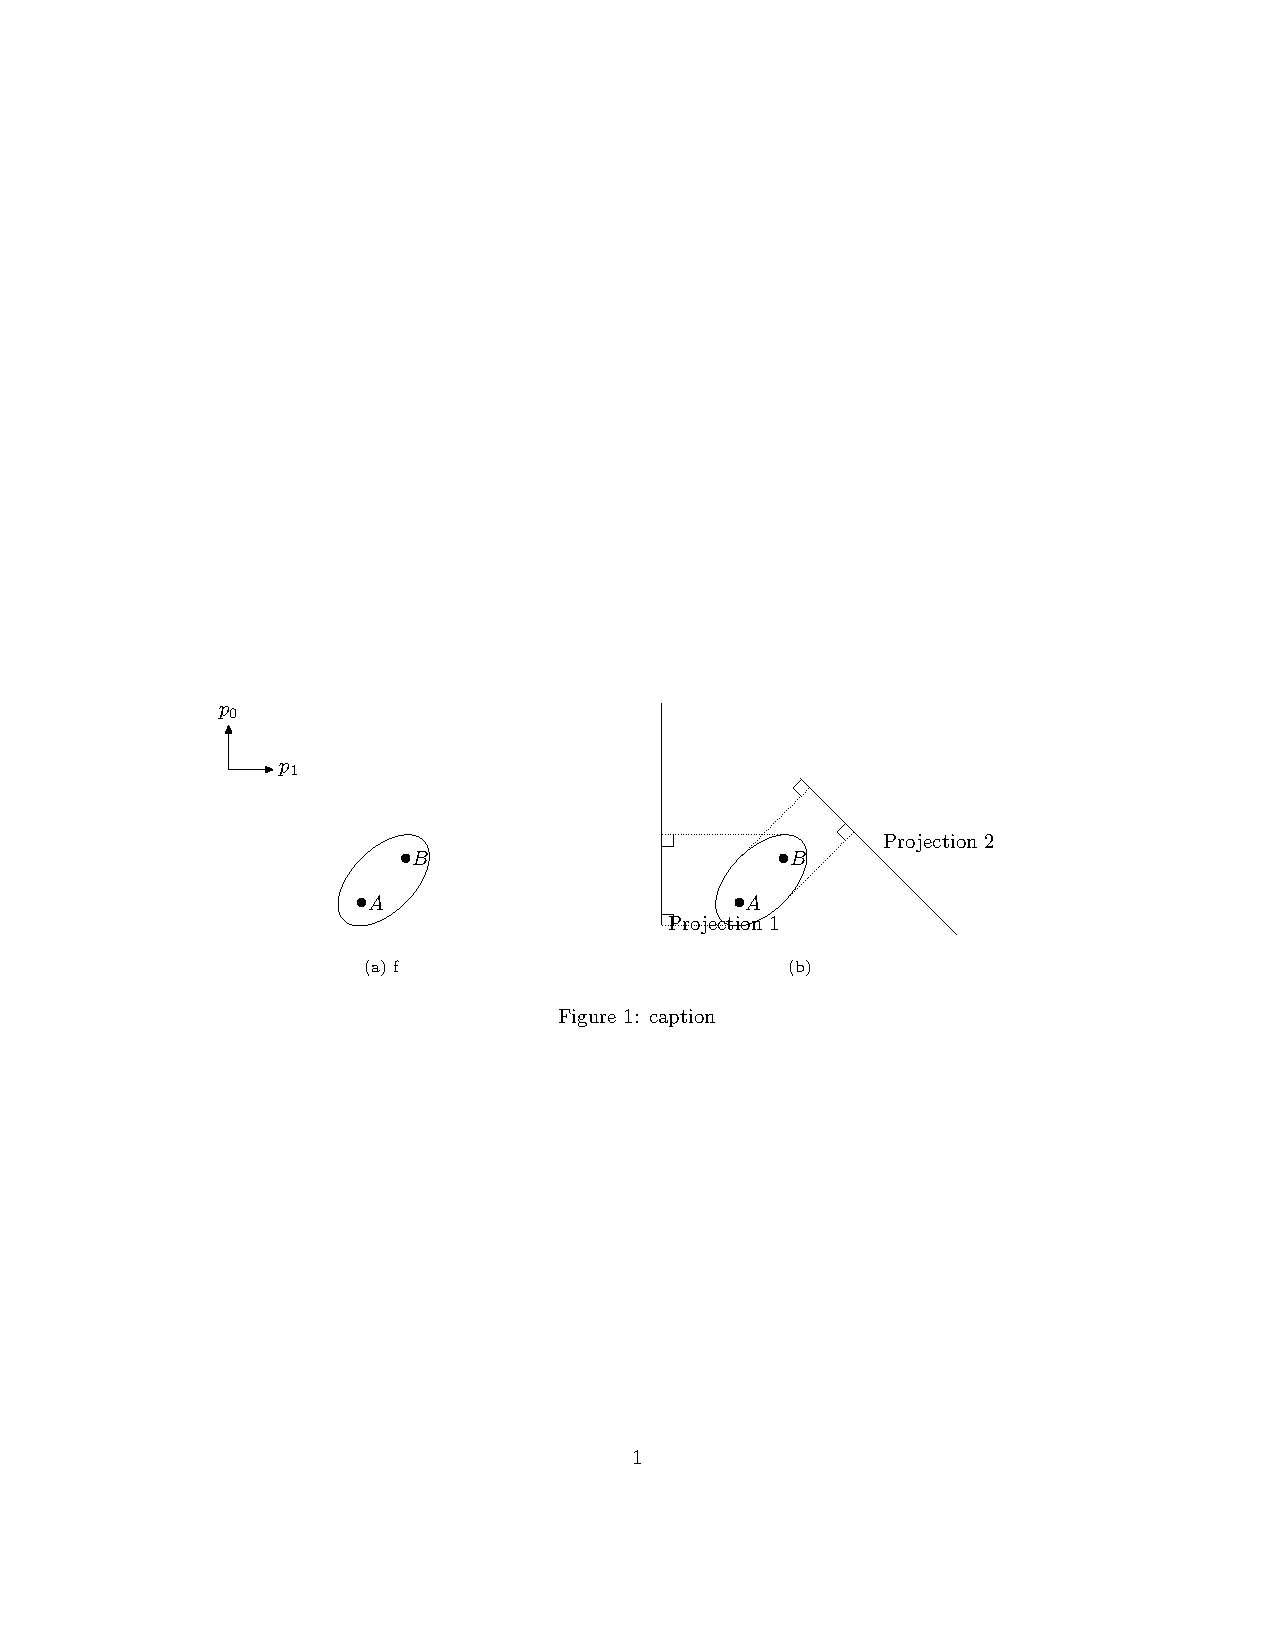
\includegraphics{measurement.4}}
%      \caption{caption}
%      \label{fig:Obs}
% \end{figure}

% \begin{figure}%[htp]
%      \centering
%      \subfigure[]{
%           \label{fig:ObsA}
%           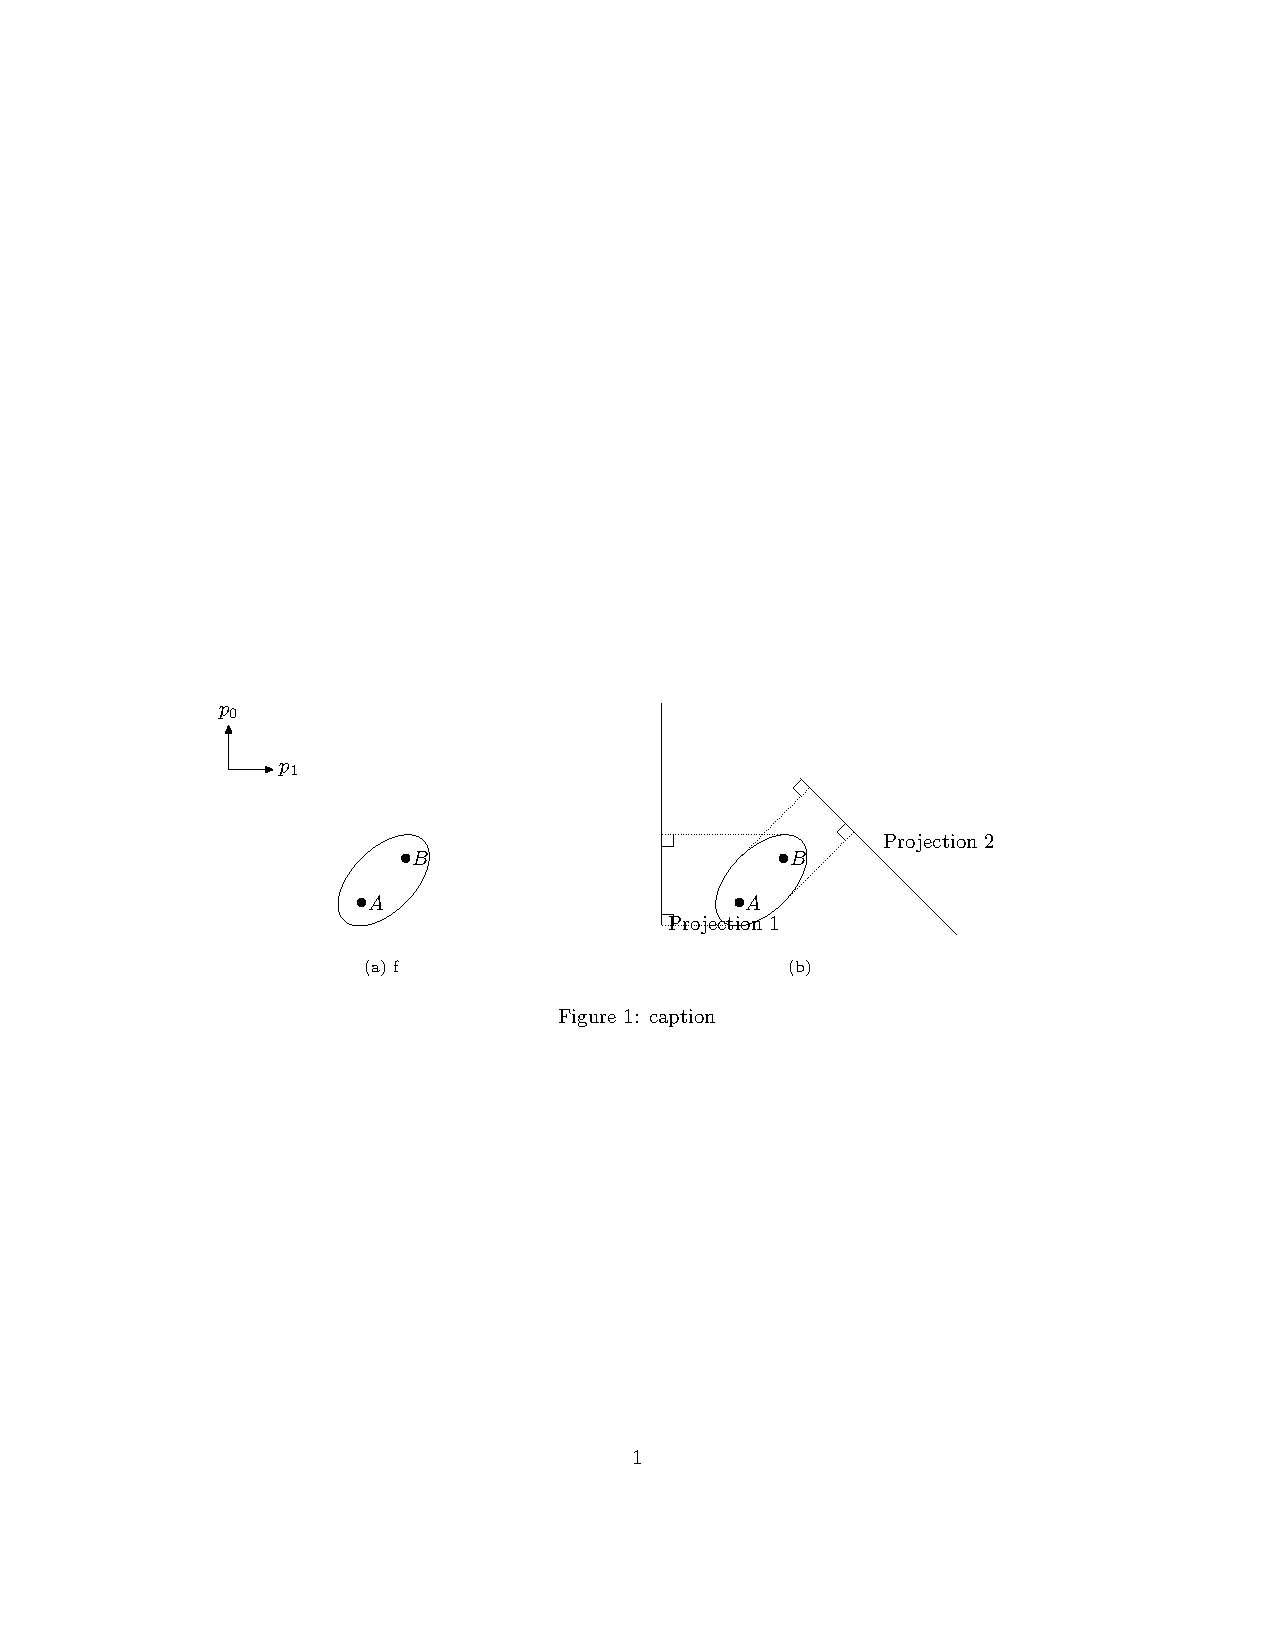
\includegraphics{measurement.5}}
%      \hspace{1cm}
%      \subfigure[]{
%           \label{fig:ObsB}
%           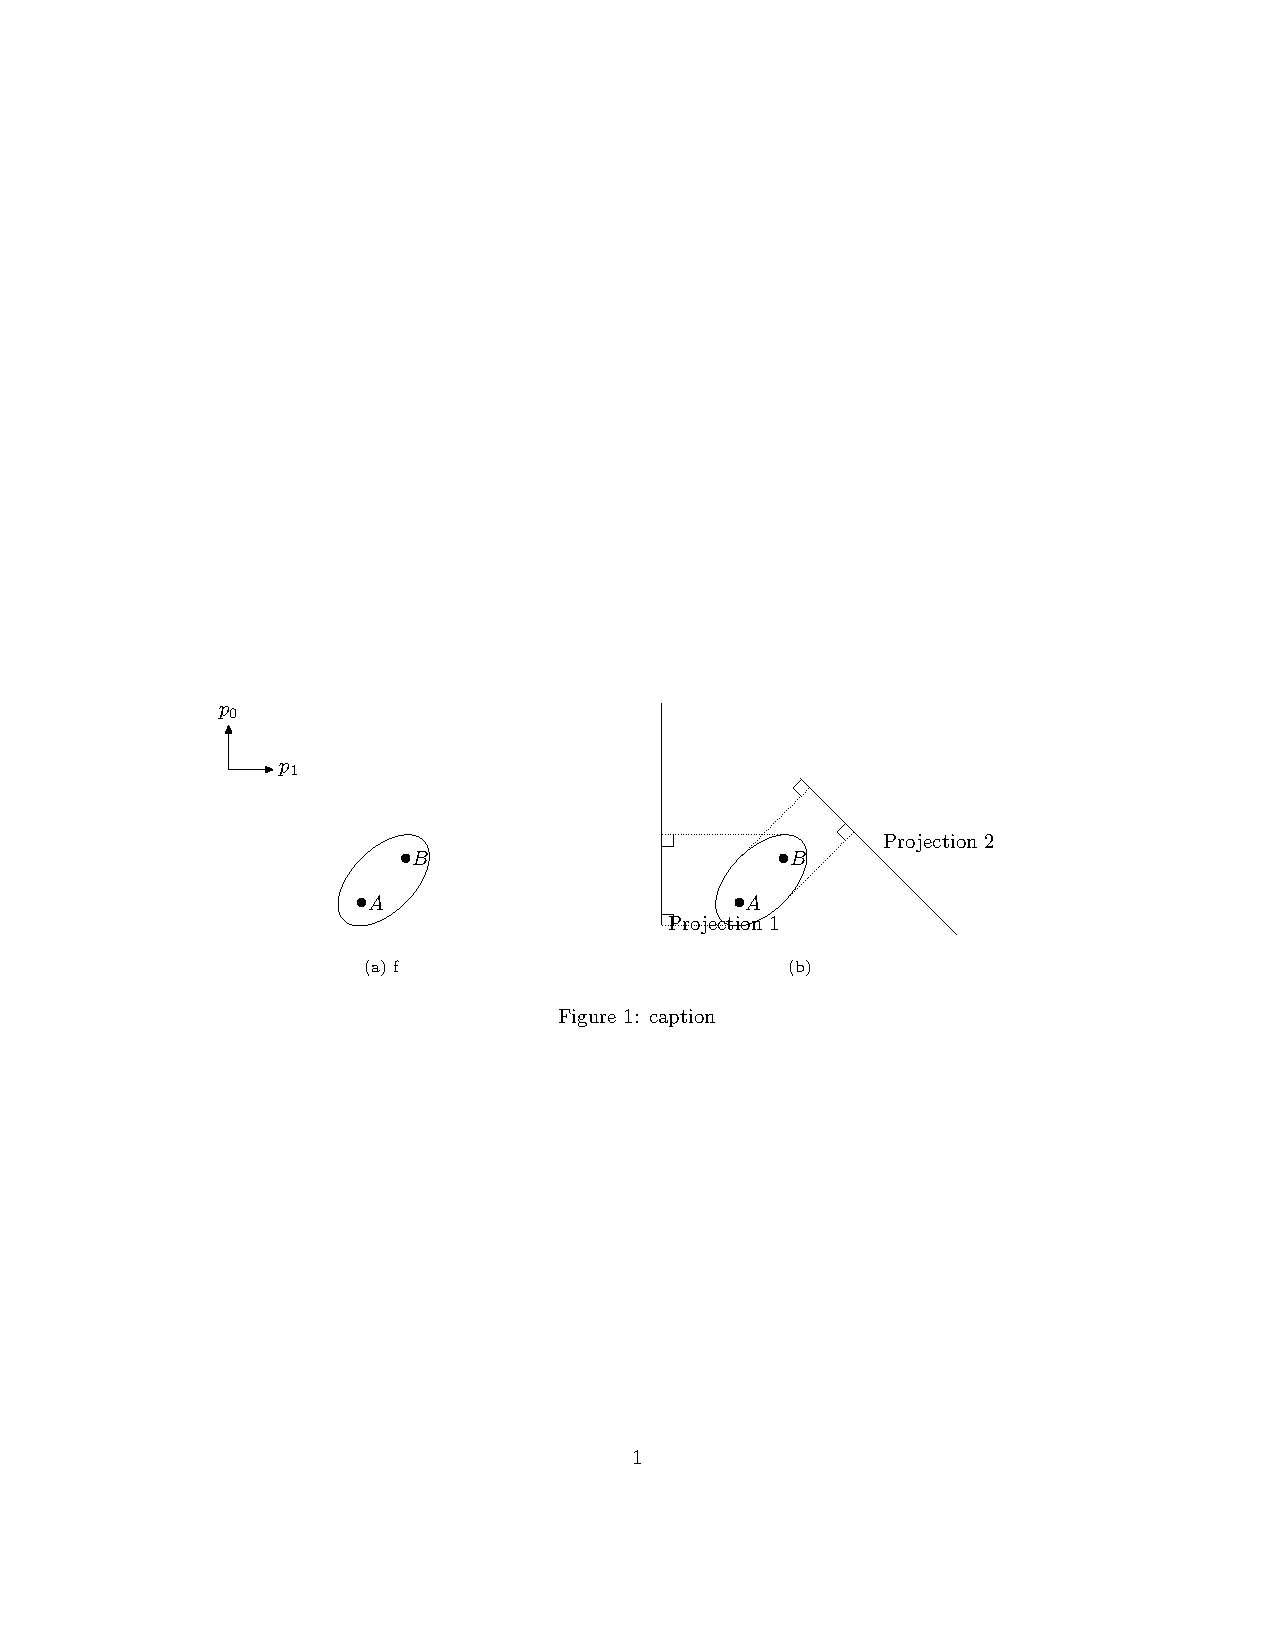
\includegraphics{measurement.6}}
%      \caption{caption}
%      \label{fig:Obs}
% \end{figure}

% \begin{figure}%[htp]
%      \centering
%      \subfigure[]{
%           \label{fig:ObsA}
%           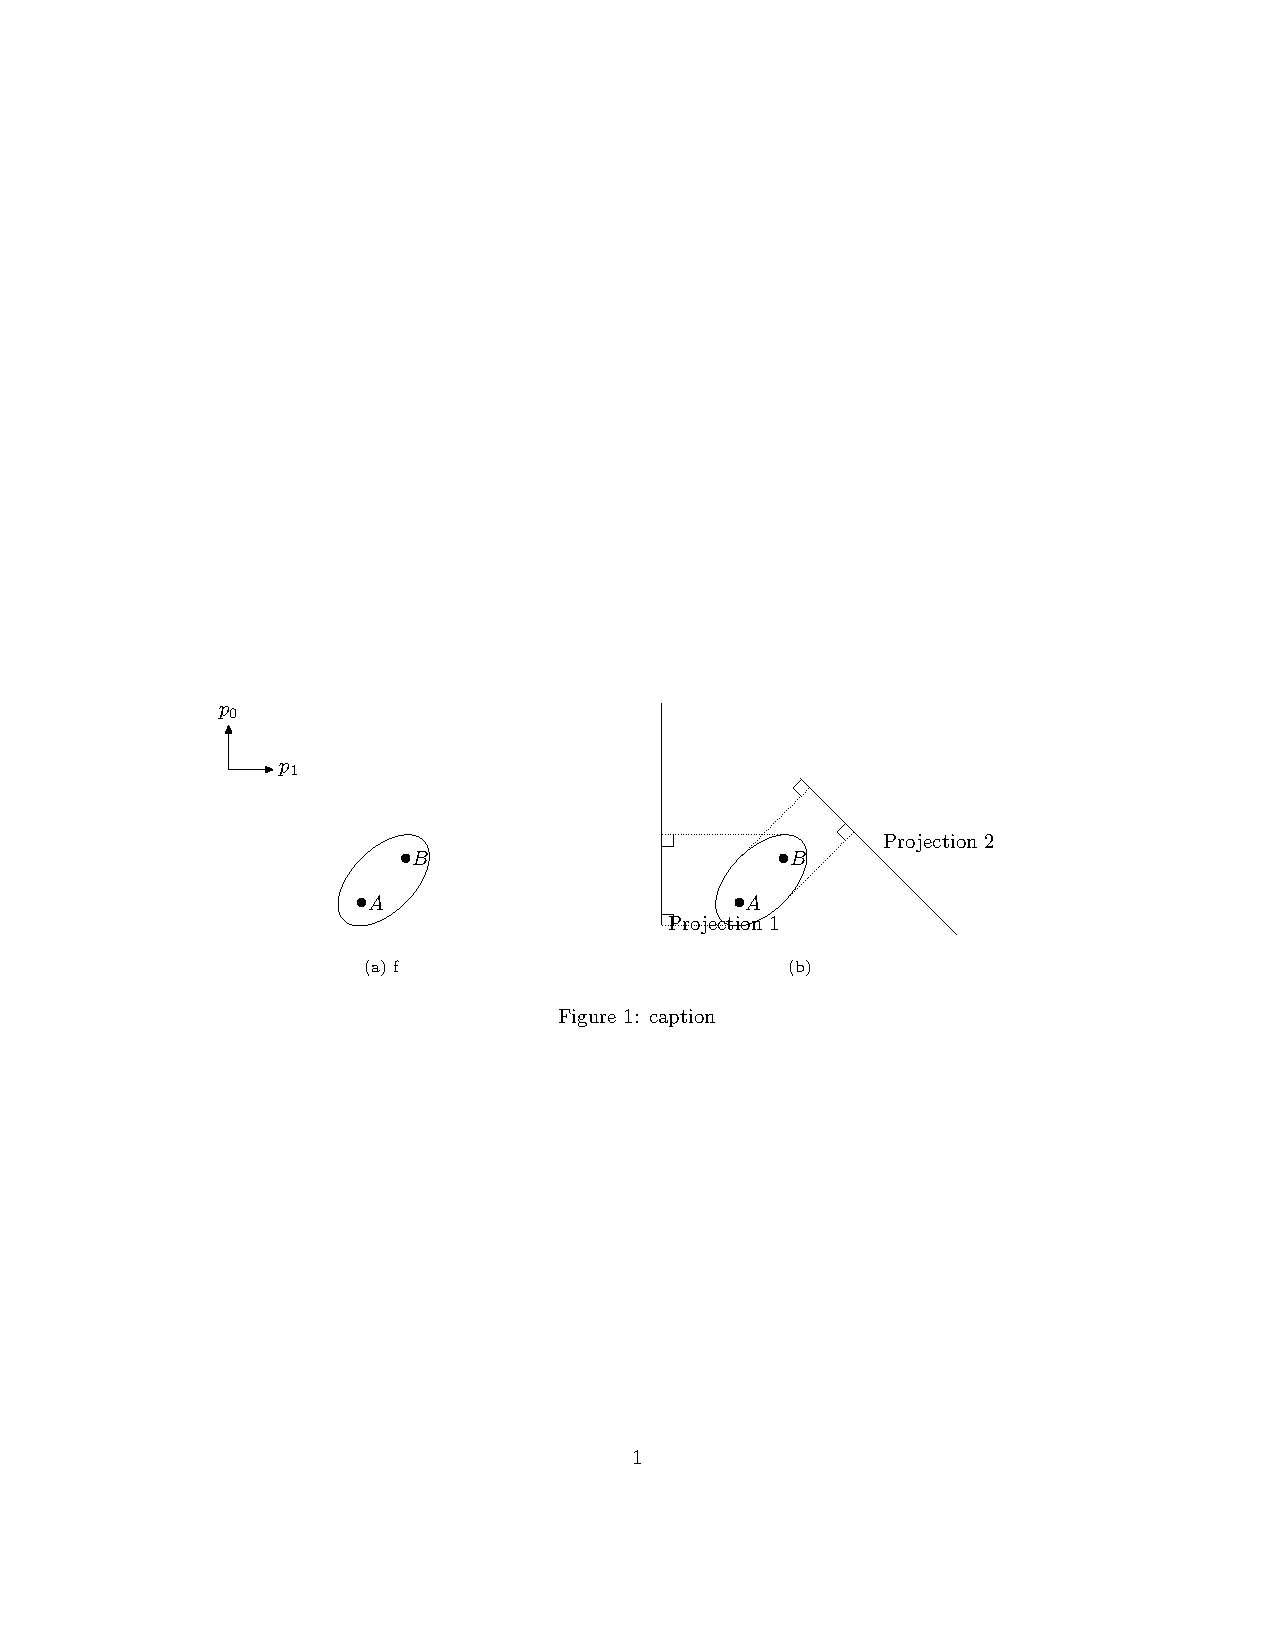
\includegraphics{measurement.7}}
%      \hspace{1cm}
%      \subfigure[]{
%           \label{fig:ObsB}
%           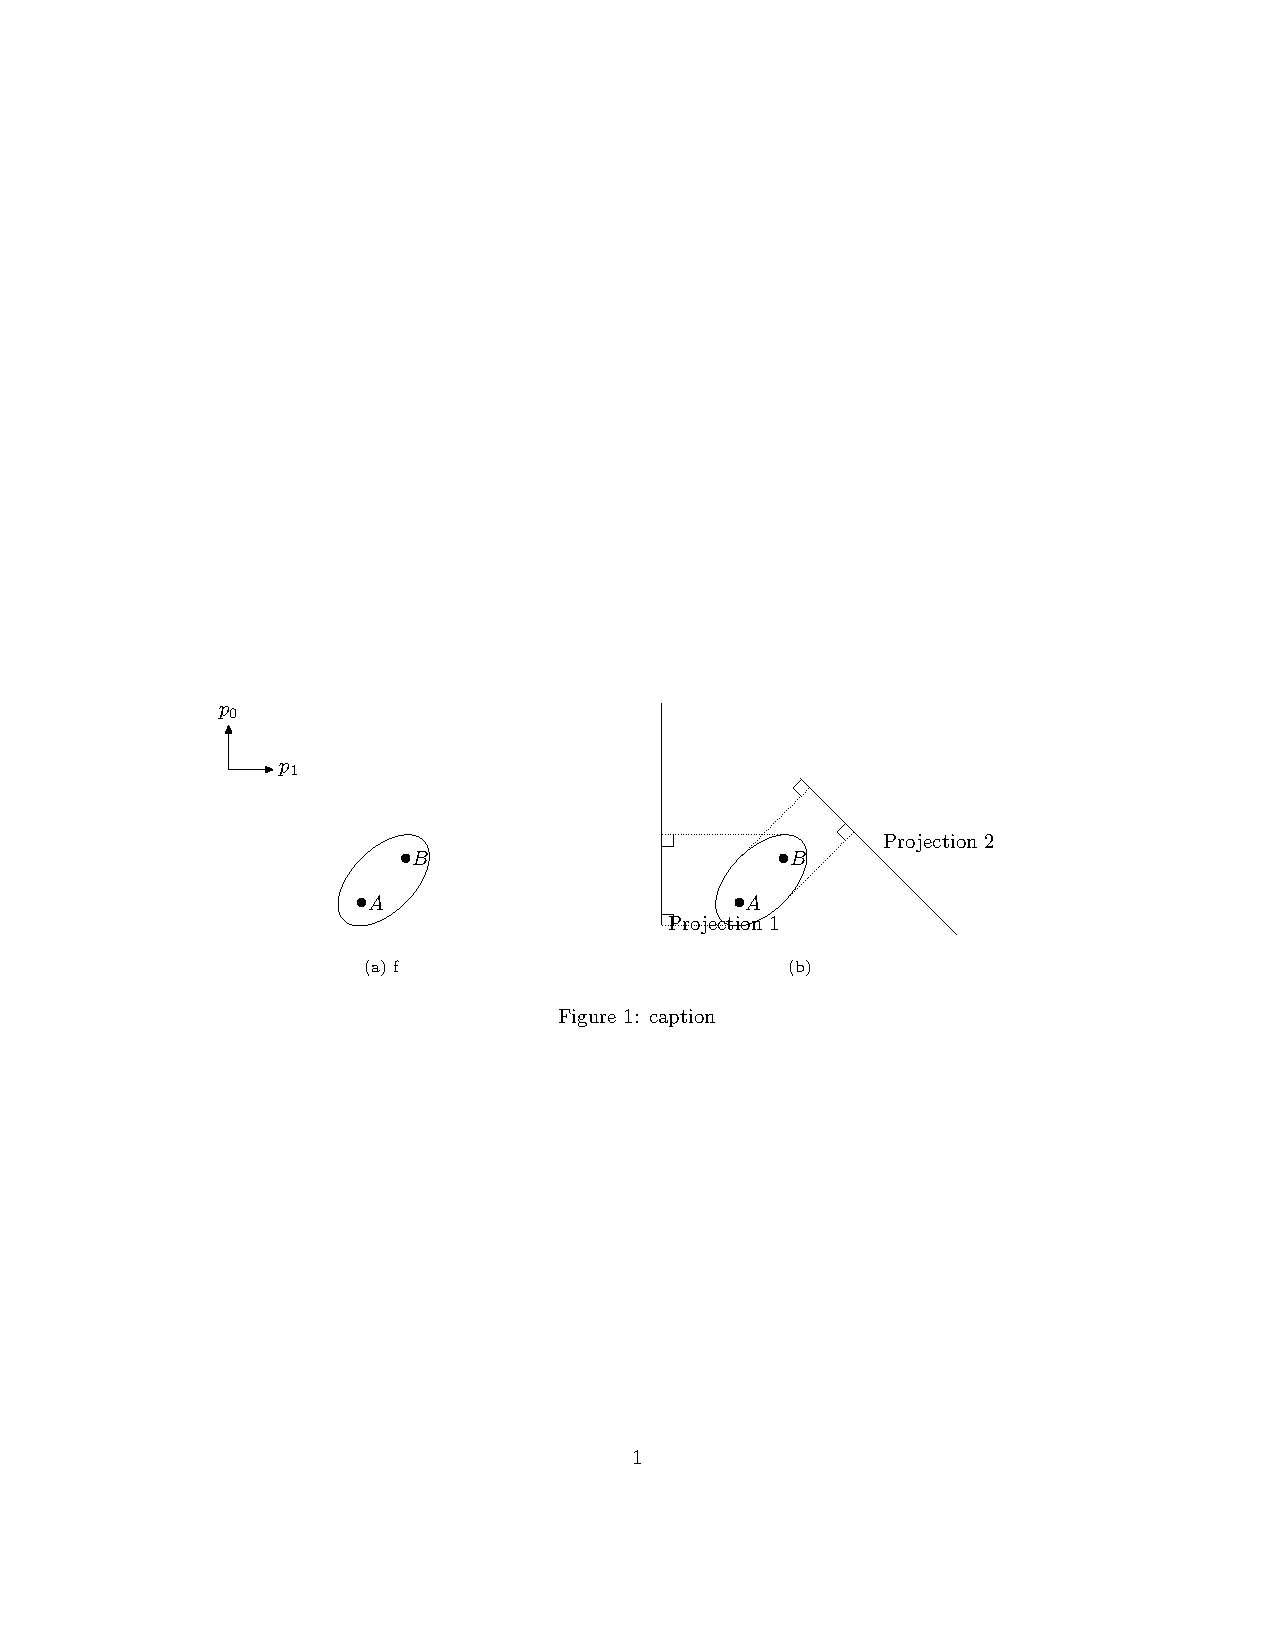
\includegraphics{measurement.8}}
%      \caption{caption}
%      \label{fig:Obs}
% \end{figure}

% \begin{figure}%[htp]
%      \centering
%      \subfigure[]{
%           \label{fig:ObsA}
%           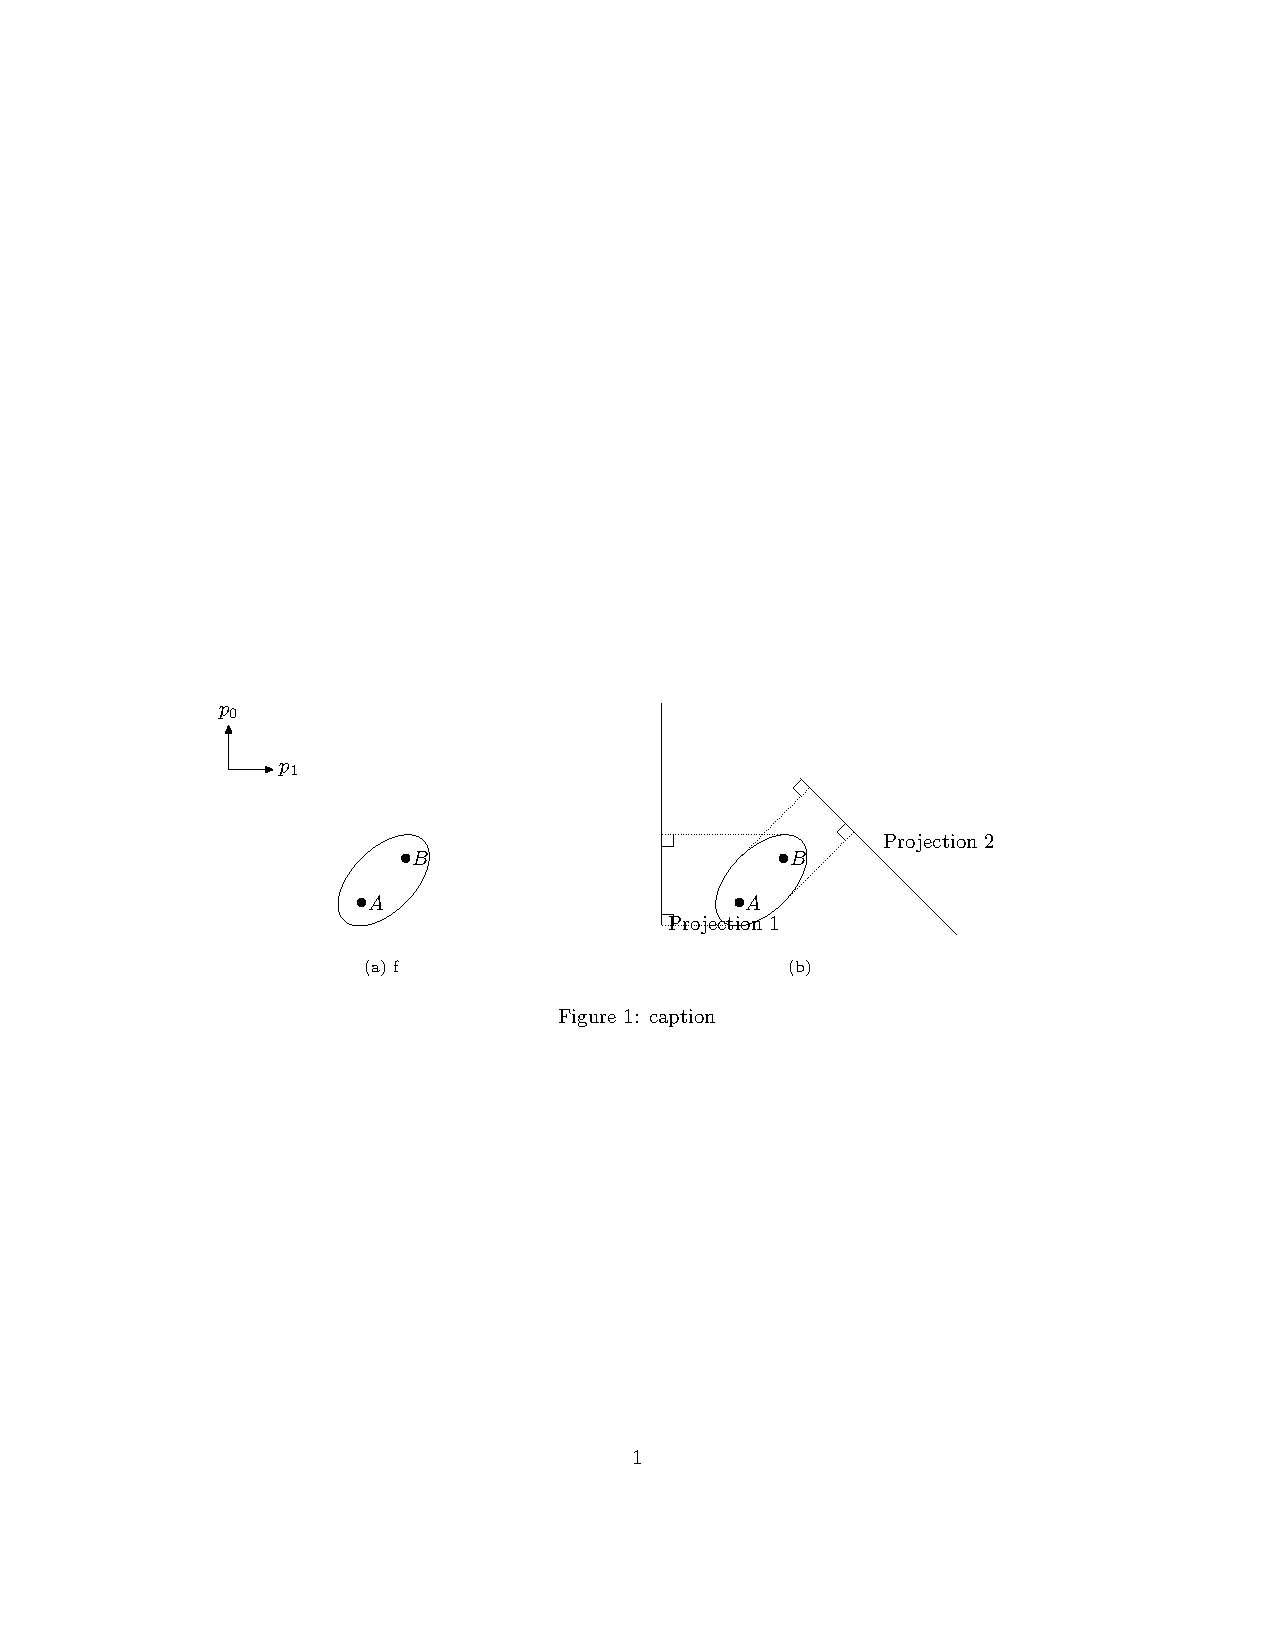
\includegraphics{measurement.9}}
%      \hspace{1cm}
%      \subfigure[]{
%           \label{fig:ObsB}
%           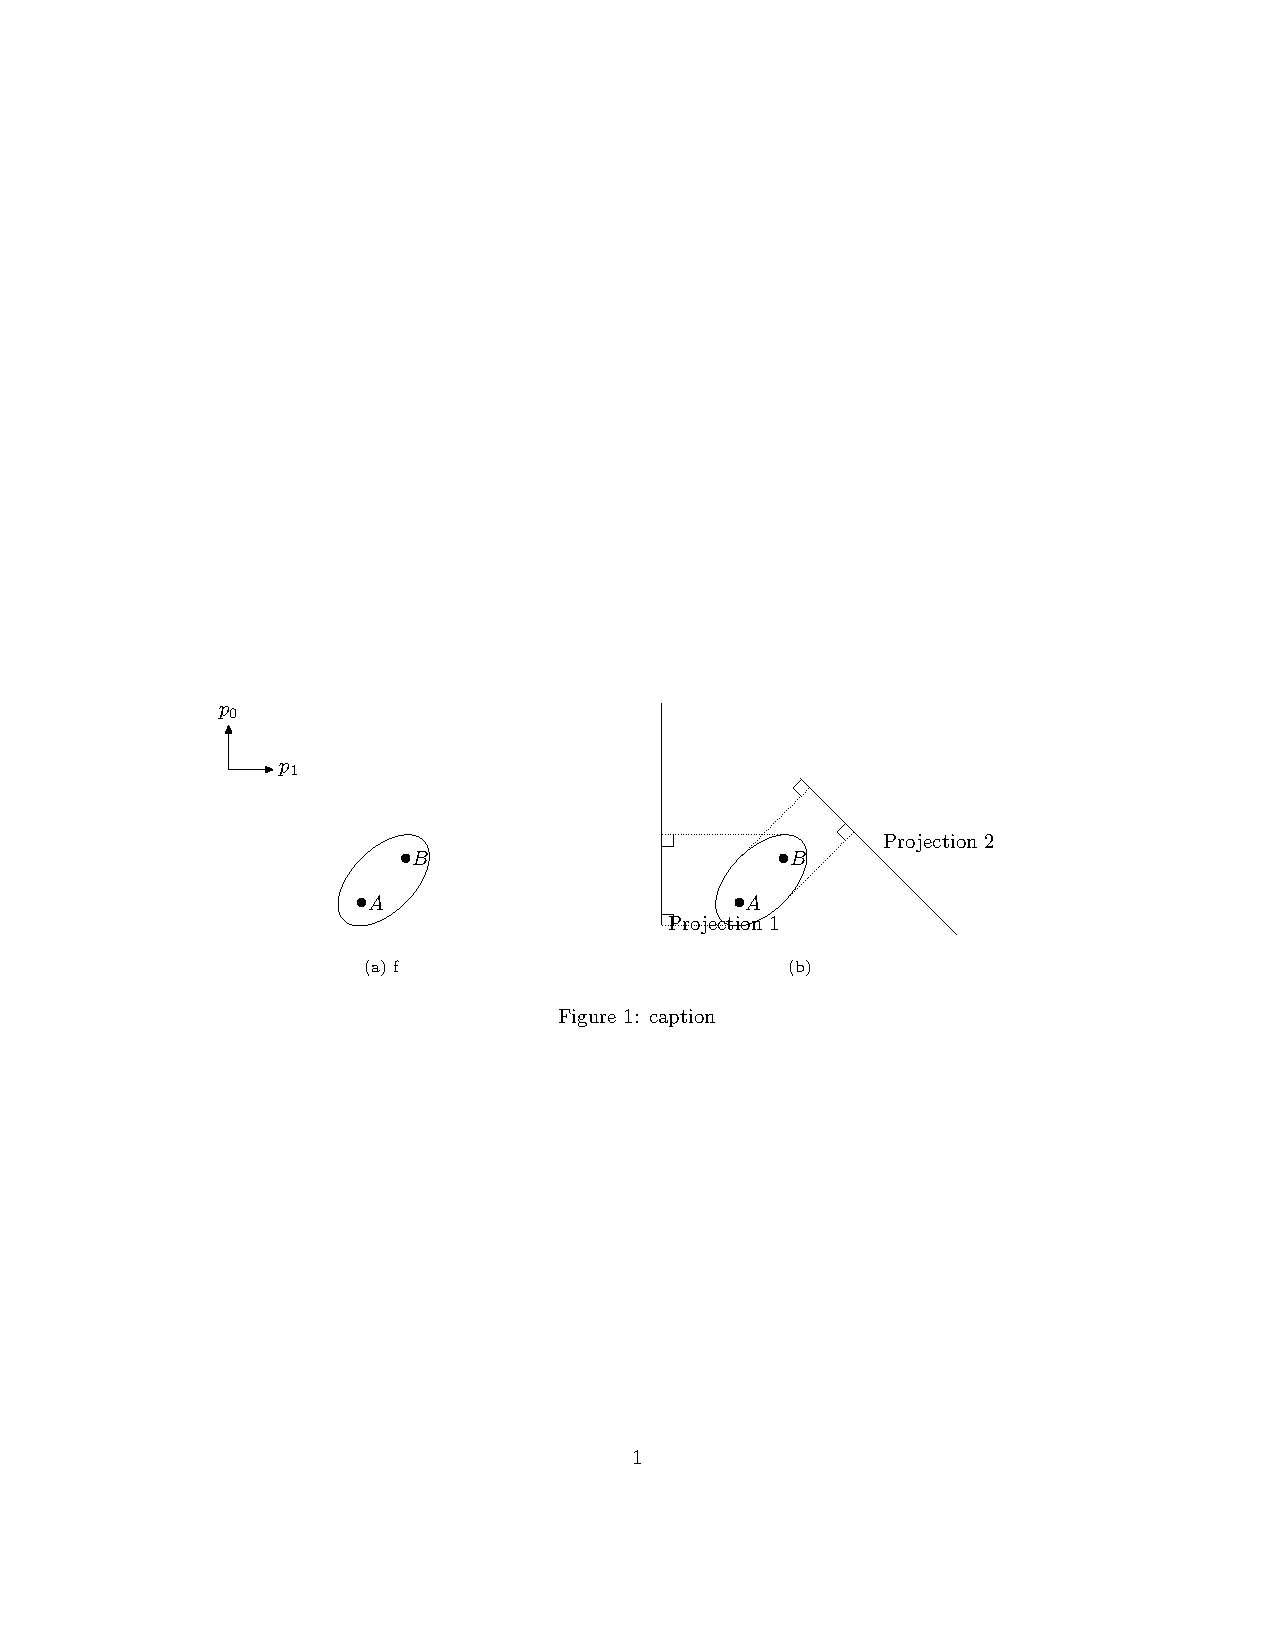
\includegraphics{measurement.10}}
%      \caption{caption}
%      \label{fig:Obs}
% \end{figure}

% %\includegraphics{lattice.3}
% %\includegraphics{lattice.4}
% %\includegraphics{lattice.5}

\end{document}
